\documentclass[10pt]{beamer}

\mode<presentation>
{
  \usetheme{Berlin}
  \setbeamertemplate{blocks}[rounded]
  \setbeamercolor{block title}{bg=gray}
  \setbeamercovered{transparent}
}

% %%% Packages %%%
% Babel and fonts
\usepackage[english]{babel}
\usepackage[utf8]{inputenc}
\usepackage{times}

% Graphics and images
\usepackage{graphicx}
\DeclareGraphicsExtensions{.pdf,.png,.jpg, .eps}
\usepackage{relsize}
\usepackage{colortbl}


% Math notation and symbols
\usepackage{mathrsfs}
\usepackage{amsthm}
\usepackage{bbold}
\usepackage{amsfonts}
\usepackage{amsmath}
\usepackage{amssymb}
% \usepackage{algorithm}
\usepackage{algpseudocode}
\usepackage{listings}

\DeclareMathOperator*{\len}{\textbf{length of }}

% \DeclareMathOperator*{\len}{\text{length of }}
% Backup slides
\usepackage{appendixnumberbeamer}

% Tables, Colums and the like
\usepackage{longtable}
\usepackage{listings}

% Hyperref
\usepackage{hyperref} 

% Boxes
\usepackage{fancybox}
\usepackage{lmodern}
\usepackage{tikz}
\usepackage{tcolorbox}
\usepackage{mdframed}	

% Custom packages
\usepackage{presmacros}
\usepackage{pdfpages}


\AtBeginSection[]
{
  \begin{frame}<beamer>
    \frametitle{Outline for section \thesection}
    \tableofcontents[currentsection]
  \end{frame}
}

\begin{document}

% \pgfdeclareimage[height=0.5 cm]{dblogo-white}{img/logo-white.png}
\setbeamertemplate{navigation symbols}{}

% \begin{frame}[plain]
%   \pgfdeclareimage[height=\paperheight]{mountain}{img/mountain.png}
%   \begin{tikzpicture}[remember picture,overlay]
%       \node[at=(current page.center)] {
% 	\pgfuseimage{mountain}
%       };
%   \end{tikzpicture}
% 
% 
%   \begin{center}
%     \usebeamerfont{title}\textcolor{white}{\inserttitle}\par
%   \end{center}
% 
% %   \begin{flushleft}
% %     \begin{small}  
% %       \textcolor{white}{presented by Cristian Consonni}
% %     \end{small}
% %   \end{flushleft}
% 
%   \begin{flushright}   
%     \pgfuseimage{dblogo-white}
%   \end{flushright}
% 
% \end{frame}

\begin{frame}
  \titlepage
\end{frame}

\begin{frame}{Outline}
  \tableofcontents
\end{frame}


\section{Intro}
\subsection[Informazioni generali]{Informazioni generali}

\begin{frame}{Chi sono}
  Cristian Consonni

  \begin{itemize}
    \item \textbf{DISI - Dipartimento di Ingegneria e Scienza dell'Informazione}
    \item \textbf{Pagina web} del laboratorio: \structure{\url{http://disi.unitn.it/~consonni/teaching}}
    \item \textbf{Email}: \structure{\url{cristian.consonni@unitn.it}}
    \item \textbf{Ufficio}: Povo 2 - Open Space 9
      \begin{itemize}
	\item Per domande: scrivetemi una mail
	\item Ricevimento: su appuntamento via mail
      \end{itemize}
  \end{itemize}
\end{frame}



\begin{frame}{Obiettivi del laboratorio}
  Obiettivi del laboratorio:
  \begin{itemize}
    \item Apprendere i fondamenti di un vero linguaggio di programmazione (Java)
    \item Svolgere il progetto
  \end{itemize}

  Obiettivi del laboratorio
  \begin{enumerate}
    \item Fare esperienza in laboratorio
    \item Raggiungere una buona manualità nell'uso degli strumenti standard
    \item Esercizi
  \end{enumerate}

\end{frame}

\pgfdeclareimage[width=0.6\paperwidth]{xkcd}{img/11th_grade.png}
\begin{frame}{Manualità (I)}
  \begin{center}
    \pgfuseimage{xkcd}
  \end{center}
  \url{https://xkcd.com/519/}
\end{frame}

\pgfdeclareimage[width=0.6\paperwidth]{abstrusegoose}{img/ars_longa_vita_brevis.png}
\begin{frame}{Manualità (II)}
  \textbf{How to Teach Yourself Programming:}\footnote{\url{http://abstrusegoose.com/249}}
  \begin{center}
    \pgfuseimage{abstrusegoose}
  \end{center}
  
\end{frame}

\begin{frame}{Slides}

  Info sulle slide:
  \begin{itemize}
    \item le slide del corso saranno rese disponibili sul sito;
    \item segnalate pure eventuali errori;
    \item cercherò di pubblicare le slide in anticipo rispetto alla lezione;
    \item queste slide sono prodotte con \LaTeX \; \texttt{Beamer} (\emph{usate} \LaTeX!);
  \end{itemize}

  Segnalazioni di materiale:
  \begin{itemize}
    \item Materiale da voi prodotto;
    \item Cose interessanti che trovate online;
    \item Possiamo valutare insieme se riutilizzarle;
  \end{itemize}
\end{frame}

\section{Java}
\subsection[Cos'è Java]{Cos'è Java}

\pgfdeclareimage[width=3cm]{javalogo}{img/javalogo.png}
\begin{frame}{Java}
 
  \begin{center}
    \pgfuseimage{javalogo}
  \end{center}
  
\end{frame}

\begin{frame}{Cos'è Java (I)}
  
  Java Language Specification (788 pagg.)\footnote{\url{https://docs.oracle.com/javase/specs/jls/se8/jls8.pdf}}
  \begin{quote}
   «The Java$^{\textregistered}$  programming  language is a general-purpose, [...] 
    class-based,  object-oriented  language.»
  \end{quote}

  Java è:
  \begin{itemize}
    \item un \textbf{linguaggio} (grammatica, vocabolario, sintassi, ecc.);
    \item linguaggio di \textbf{programmazione};
    \item general-purpose (vs domain-specific, e.g. \textit{SQL});
    \item orientato agli \textbf{oggetti} (attributi, metodi);
    \item class-based (\textbf{classe}, ereditarietà);
  \end{itemize}

\end{frame}

\begin{frame}{Cos'è Java (II)}
  
  Altre caratteristiche di Java:
  \begin{itemize}
    \item \textbf{imperativo} (vs. funzionale vs. logico);
  \end{itemize}
\end{frame}

{
  \setbeamercolor{background canvas}{bg=}
  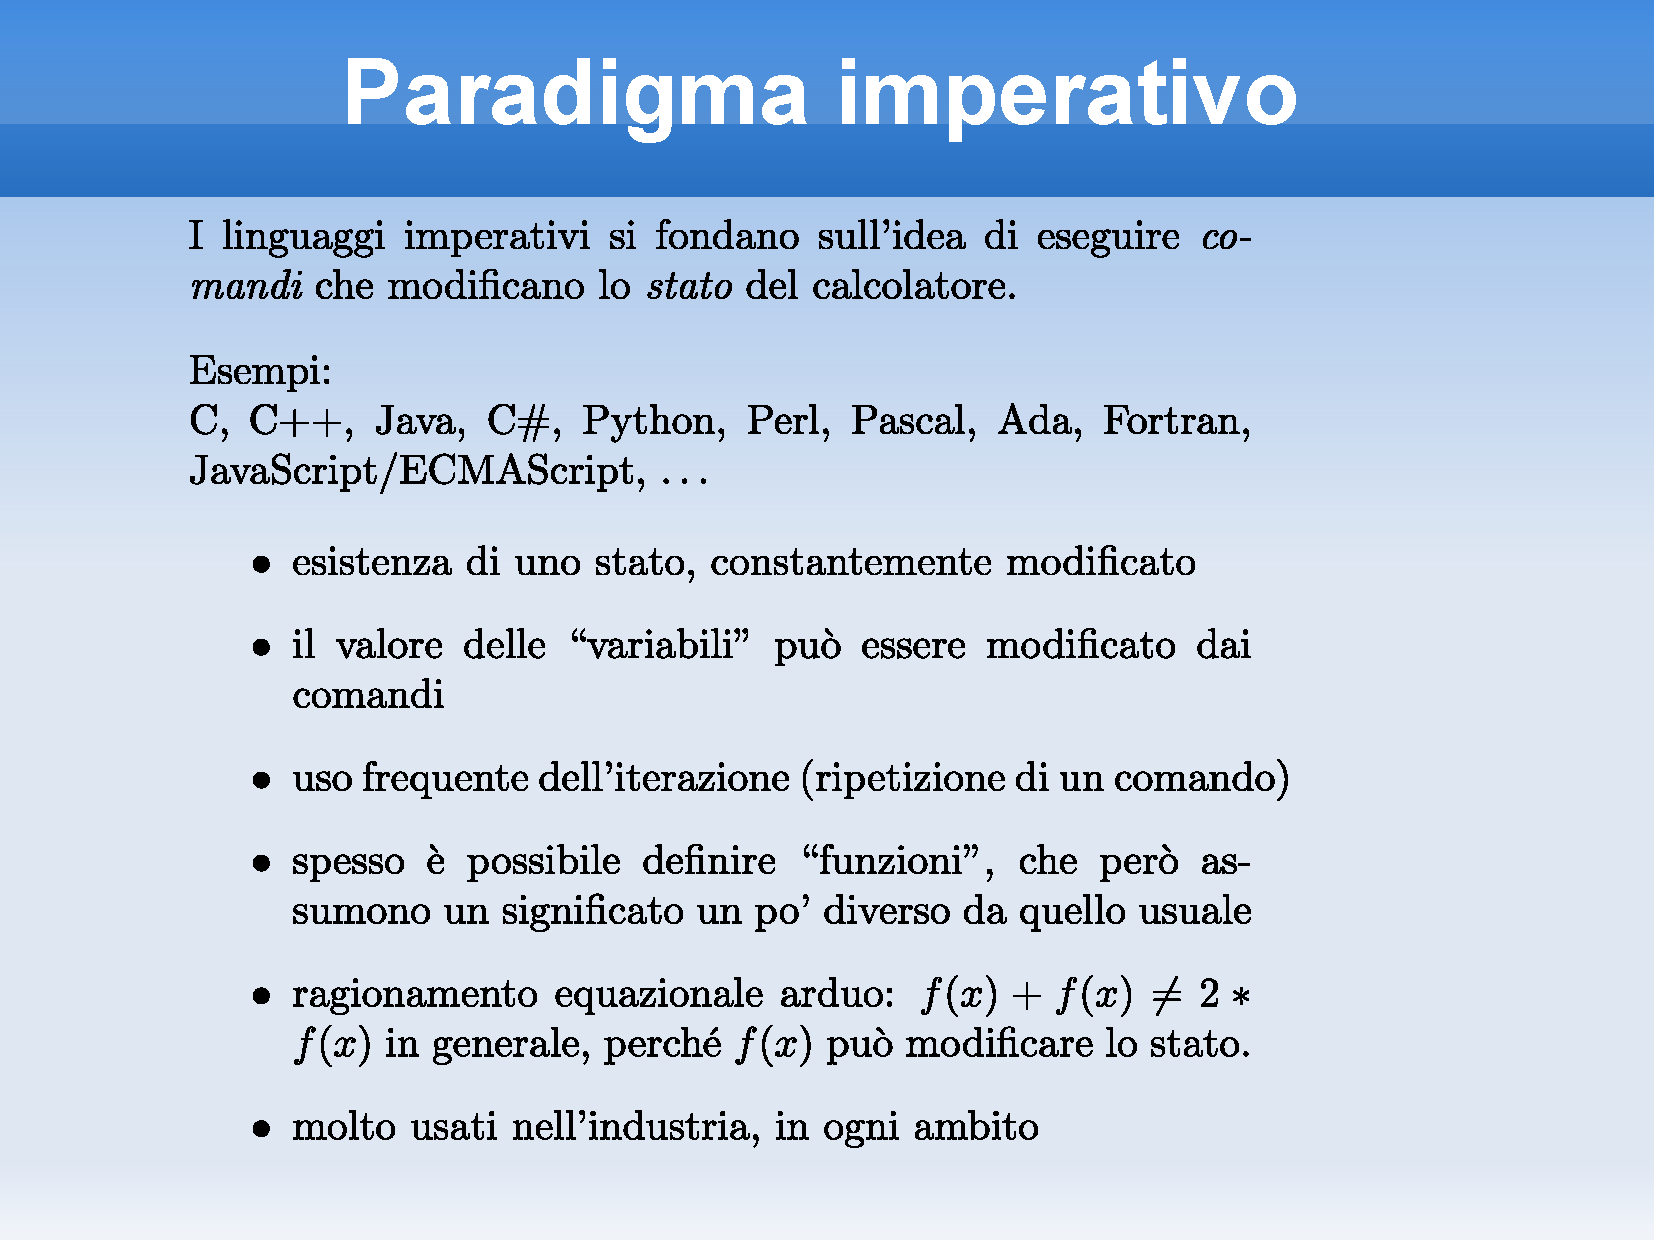
\includepdf[pages={1}]{img/imperativo.pdf}
}

\begin{frame}{Cos'è Java (II)}
  
  Altre caratteristiche di Java:
  \begin{itemize}
    \item \textbf{imperativo} (vs. funzionale vs. logico);
    \item \textbf{compilato} (vs. interpretato);
    \item \textbf{fortemente tipizzato}, \emph{strongly typed} (vs. debolmente tipizzato)
    \item Molto usato in svariati ambiti;
    \item ...
  \end{itemize}
\end{frame}

\subsection[Altri linguaggi]{Altri linguaggi}

\begin{frame}{Altri linguaggi}

  Esistono moltissimi altri linguaggi:
  \begin{itemize}
    \item ad es. linguaggi di markup (e.g. HTML, XML, TeX)
    \item altri linguaggi \textbf{di programmazione}: C, C++, python,
  go, Scala, Prolog, Perl, $\dots$

  \end{itemize}
\end{frame}

\pgfdeclareimage[width=0.5\paperwidth]{hello_c}{img/hello_c.png}
\begin{frame}{Altri linguaggi (II)}
  \textbf{C}:
  \begin{center}
    \pgfuseimage{hello_c}
  \end{center}
\end{frame}

\pgfdeclareimage[width=0.5\paperwidth]{hello_py}{img/hello_py.png}
\begin{frame}{Altri linguaggi (III)}
  \textbf{Python}:
  \begin{center}
    \pgfuseimage{hello_py}
  \end{center}
\end{frame}

\pgfdeclareimage[width=0.5\paperwidth]{hello_java}{img/hello_java.png}
\begin{frame}{Altri linguaggi (IV)}
  \textbf{Java}:
  \begin{center}
    \pgfuseimage{hello_java}
  \end{center}
\end{frame}


\pgfdeclareimage[width=0.5\paperwidth]{hello_c_exe}{img/hello_c_exe.png}
\begin{frame}{Altri linguaggi (V)}
  \textbf{C}:
  \begin{center}
    \pgfuseimage{hello_c_exe}
  \end{center}
\end{frame}

\pgfdeclareimage[width=0.5\paperwidth]{hello_py_exe}{img/hello_py_exe.png}
\begin{frame}{Altri linguaggi (VI)}
  \textbf{Python}:
  \begin{center}
    \pgfuseimage{hello_py_exe}
  \end{center}
\end{frame}

\pgfdeclareimage[width=0.5\paperwidth]{hello_java_exe}{img/hello_java_exe.png}
\begin{frame}{Altri linguaggi (VII)}
  \textbf{Java}:
  \begin{center}
    \pgfuseimage{hello_java_exe}
  \end{center}
\end{frame}

\pgfdeclareimage[width=0.5\paperwidth]{hello_c_comp}{img/hello_c_comp.png}
\begin{frame}{Altri linguaggi (VIII)}
  \textbf{C (bynary)}:
  \begin{center}
    \pgfuseimage{hello_c_comp}
  \end{center}
\end{frame}

\pgfdeclareimage[width=0.75\paperwidth]{hello_java_comp}{img/hello_java_comp.png}
\begin{frame}{Altri linguaggi (IX)}
  \textbf{Java (bytecode)}:
  \begin{center}
    \pgfuseimage{hello_java_comp}
  \end{center}
\end{frame}

\begin{frame}{Pseudocodice}

  Per esprimere un algoritmo senza adottare una sintassi legata ad un particolare
  linguaggio si usa lo \textbf{pseudocodice}:
    \begin{algorithmic}[1]
      
      \State $sum \gets 0$
      \For{$i \gets 1$ to $N$}
	\For{$j \gets 0$ to $i$}
	  \If{$i \mod 2 = 0$}
	    \State $sum \gets sum + 1$ 
	  \EndIf
	\EndFor
      \EndFor
    \end{algorithmic}

\end{frame}

\begin{frame}{Pseudocodice (II)}

  Per esprimere un algoritmo senza adottare una sintassi legata ad un particolare
  linguaggio si usa lo \textbf{pseudocodice}:
  
  (Esempio di dichiarazione di funzioni)
  \begin{algorithmic}[H]
    \Function{InsertionSort}{Array $x$}
      \For{$i \gets \len{A}$}
	\State $value \gets A[i]$
	\State $j \gets i - 1$
	\While{$j \geq 0$ $\wedge$ $A[j] > value$}
	  \State $A[j + 1] \gets A[j]$
	  \State $j \gets j-1$
	\EndWhile
      \EndFor
    \EndFunction
  \end{algorithmic}

\end{frame}
 
\section{Variabili}
\subsection[Definizione ed esempi]{Definizione ed esempi}

\begin{frame}{Variabili (I)}

  Variabile\footnote{da \url{https://en.wikipedia.org/wiki/Variable_(computer_science)}}:
  \begin{quote}
    «In computer programming, a \textbf{variable} or scalar is a \alert<2->{storage location}
     paired with an \alert<3->{associated symbolic name (an identifier)}, which contains some
     known or unknown quantity of information referred to as a \alert<4->{value}.»
  \end{quote}

\end{frame}

\begin{frame}{Variabili (II)}

  Esempi:   
    \begin{columns}[T] % contents are top vertically aligned
      \begin{column}[T]{5cm} % each column can also be its own environment
	\begin{enumerate}[<+->]
	  \item un intero:
	  \begin{itemize}
	    \item \texttt{\textbf{int} i = 0;}
	    \item Pseudocodice $i \gets 0$
	  \end{itemize}
	  \item un numero con la virgola:
	  \begin{itemize}
	    \item \texttt{\textbf{double} pi = 3.14;}
	    \item (usate \texttt{Math.PI} per $\pi$)
	  \end{itemize}
	  \item un (singolo) carattere:
	  \begin{itemize}
	    \item \texttt{\textbf{char} k = \structure{'c'};}
	  \end{itemize}
	\end{enumerate}
      \end{column}
      \begin{column}[T]{7cm} % alternative top-align that's better for graphics
	\begin{enumerate}[<+->]
	  \setcounter{enumi}{3}
	  \item un \emph{valore booleano}:
	  \begin{itemize}
	    \item \texttt{\textbf{bool} val1 = \textbf{true};}
	    \item \texttt{\textbf{bool} val2 = \textbf{false};}
	  \end{itemize}
	  \item una \emph{stringa} di caratteri:
	  \begin{itemize}
	    \item \texttt{\textbf{String} yoda = \structure{"There is no try!"};}
	  \end{itemize}
	\end{enumerate}
      \end{column}
    \end{columns}
\end{frame}

\begin{frame}{Variabili (III)}

  Una variable:
  \begin{itemize}
    \item Sono un ``\emph{contenitore}'' di informazioni (= un certo numero di bytes allocati nella 
	  memoria volatile del computer (RAM));
    \item Contraddistinte da un identificatore, negli esempi di prima \texttt{i}, \texttt{pi}, 
	  \texttt{yoda}, $\dots$
	  (\emph{case sensitive} \texttt{pippo} $\neq$ \texttt{Pippo} $\neq$ \texttt{PIPPO}); 
    \item Nei linguaggi fortemente tipizzati hanno un \textbf{tipo}, negli esempi di prima 
	  \texttt{\textbf{int}}, \texttt{\textbf{double}}, \texttt{\textbf{String}}, $\dots$;
  \end{itemize}

\end{frame}

\subsection[Dichiarazione e assegnamento]{Dichiarazione e assegnamento}

\begin{frame}{Dichiarazione e assegnamento}

  Le Variabilo possono essere create con la \textbf{dichiarazione}:
  \begin{itemize}
    \item \textbf{\structure{dichiarazione}}: \texttt{\textbf{int} i;} (\emph{specifica} il tipo di un identificatore);
    \item \textbf{\structure{assegnamento}}:  \texttt{i = 1;} (\emph{assegna} un valore a un identificatore);
    \item \textbf{\structure{inizializzazione}}: primo assegnamento \texttt{\textbf{int} i = 1;} (dichiarazione + inizializzazione);
  \end{itemize}

\end{frame}


\section{Operatori}
\subsection[Definizione]{Definizione}


\begin{frame}{Operatori (I)}
  
  Definizione:\footnote{da \url{https://en.wikipedia.org/wiki/Operator_(computer_programming)}}
  \begin{quote}
    «[Operator are] constructs which behave generally like functions, but which differ syntactically 
      or semantically from usual functions»
  \end{quote}
\end{frame}

\begin{frame}{Operatori (II)}

  Gli operatori:
  \begin{itemize}
    \item funzioni disponibili in maniera predefinita all'interno di un linguaggio (ce ne sono molte altre);
    \item ritornano un risultato che avrà un certo \textbf{tipo};
    \item \textbf{notazione infissa} (\emph{infix notation}) operatore inserito tra gli operandi, ad es. \texttt{2 + 2};
    \item \textbf{arietà} (o \textbf{adicità}) (numero di argomenti, v. \emph{funzione variadica}):
      \begin{itemize}
	\item \textbf{binari}: \texttt{$+$} (addizione), \texttt{$>$} (maggiore), \texttt{$<=$} (minore uguale),
	      \texttt{$\&$} (\emph{bitwise and}), \texttt{$=$} (assegnamento), \texttt{$[]$} (\emph{bitwise and});
	\item \textbf{unari}: \texttt{$-$} (sottrazione), \texttt{$\!$} (negazione), \texttt{$++$} (decremento);
	\item (in alcuni linguaggi \alert{ma non in Java} tramite l'\emph{overload} possono essere estese le funzionalità
	      di un operatore);
      \end{itemize}  
  \end{itemize}
\end{frame}

\subsection[Operatori aritmetici]{Operatori aritmetici e booleani}

\begin{frame}{Operatori aritmetici}
  \begin{columns}[T]
    \begin{column}[T]{4cm}
      Date tre variabili:
      \begin{itemize}
	\item \texttt{\textbf{int} x = 12;}
	\item \texttt{\textbf{int} y = 5;}
	\item \texttt{\textbf{int} z = 0;}
      \end{itemize}
    \end{column}
    \begin{column}[T]{7cm}
      \begin{itemize}[<+->]
	\item \texttt{$+$}, \texttt{$-$}, \texttt{$*$} funzionano come vi aspettate
	\item \texttt{$/$} \alert{\textbf{attenzione!}} \texttt{k = x / y;}
	\item \texttt{$\%$} modulo (resto della divisione)
      \end{itemize}
    \end{column}
  \end{columns}
\end{frame}

\newcolumntype{C}[1]{>{\centering\let\newline\\\arraybackslash\hspace{0pt}}m{#1}}
\begin{frame}{Operatori booleani}
  Anche in questo caso funziona tutto normalmente:
  \begin{table}[h]
  \centering
    \begin{tabular}{|c|c|C{1.5cm}|C{1.5cm}|C{1.5cm}|}
      \hline
      $p$ & $q$ & $\neg p$ \newline (\texttt{!p}) & $p \wedge q$  \newline (\texttt{p \&\& q}) & $p \vee q$ \newline (\texttt{p || q}) \\ \hline
      $T$ & $T$ & $F$     & $T$       & $T$ \\ \hline
      $T$ & $F$ & $F$     & $F$       & $T$ \\ \hline
      $F$ & $T$ & $T$     & $F$       & $T$ \\ \hline
      $F$ & $F$ & $T$     & $F$       & $F$ \\ \hline
    \end{tabular}
  \end{table}

  \begin{itemize}[<+->]
    \item \alert{\textbf{attenzione!}} ai valori di verità delle variabili non booleane;
    \item \texttt{$==$} operatore di confronto;
    \item \texttt{a.equals(b)} confronto tra stringhe (\texttt{\texttt{String}});
  \end{itemize}

\end{frame}




 
\section{Eclipse}
\subsection[Installazione]{Installazione}

\pgfdeclareimage[width=5cm]{eclipselogo}{img/eclipselogo.png}
\begin{frame}{Eclipse (I)}

  Eclipse è un \textbf{ambiente di sviluppo integrato} (\emph{IDE}) multi-linguaggio e multipiattaforma.
  \begin{center}
    \pgfuseimage{eclipselogo}
  \end{center}

\end{frame}

\begin{frame}{Eclipse (II)}

  Eclipse è un \textbf{ambiente di sviluppo integrato} (\emph{IDE}) multi-linguaggio e multipiattaforma.
  
  \begin{itemize}
    \item software \textbf{libero} e \textbf{open source};
    \item versione 1.0 rilasciata nel 2001, versione stabile 4.5.0 \emph{Mars} (giugno 2015), voi avete 4.4.0 \emph{Luna};
    \item multipiattaforma;
    \item estendibile con \textbf{plugins};
  \end{itemize}
\end{frame}

\begin{frame}{Scaricare e installare Eclipse}

  \begin{enumerate}
    \item Scaricare Java \textbf{JDK} (\emph{Java Development Kit}) \url{http://www.oracle.com/technetwork/java/javase/downloads/index.html};
    \item Scaricare Eclipse \url{https://www.eclipse.org/downloads/};
    \begin{itemize}
      \item \url{https://www.cs.umd.edu/eclipse/}
    \end{itemize}
  \end{enumerate}
\end{frame}

\begin{frame}{Verificare che l'installazione di Java è andata a buon fine}

  Aprendo un \textbf{terminale} (o \emph{shell}) (*nix) o ``prompt dei comandi'' (Windows): \newline
  \texttt{
     \$ java -version \newline                                                                                                          
     java version "1.8.0\_60" \newline
     Java(TM) SE Runtime Environment (build 1.8.0\_60-b27) \newline
     Java HotSpot(TM) 64-Bit Server VM (build 25.60-b23, mixed mode)
     }

\end{frame}
 

\begin{frame}{Altre IDE}

  Esistono molte altre IDE:
  \begin{enumerate}
    \item \textbf{NetBeans}: \url{https://netbeans.org/}
    \item \textbf{IntelliJ IDEA}: \url{https://www.jetbrains.com/idea/}
  \end{enumerate}
\end{frame}
 
\subsection[Creazione progetto]{Creazione progetto}

\pgfdeclareimage[width=6cm]{eclipse_splash}{img/eclipse/eclipse_mars_splash_screen.png}
\begin{frame}{Avvio di Eclipse (I)}
  \begin{center}
    \pgfuseimage{eclipse_splash}
  \end{center}
\end{frame}

\pgfdeclareimage[width=6cm]{workspace}{img/eclipse/workspace.png}
\begin{frame}{Workspace}
  \textbf{Workspace}:
  \begin{center}
    \pgfuseimage{workspace}
  \end{center}
\end{frame}
% {
%   \setbeamercolor{background canvas}{bg=}
%   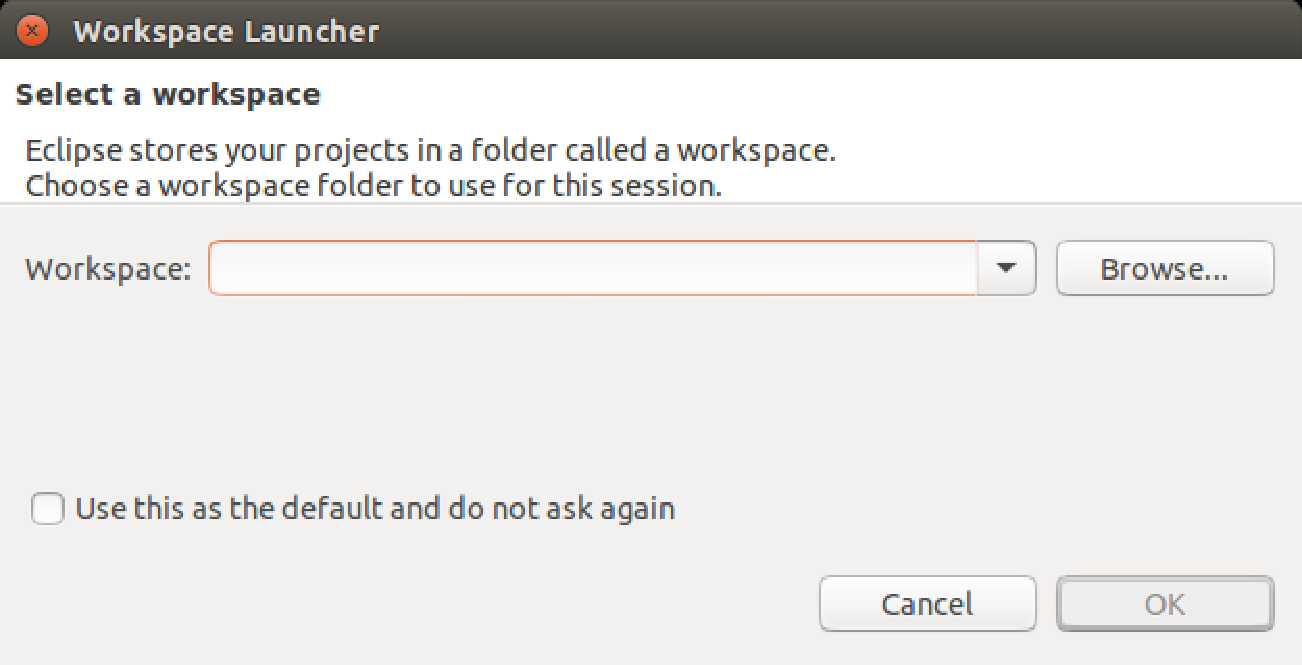
\includepdf[pages={1}]{img/eclipse/workspace.pdf}
% }

% \pgfdeclareimage[height=\paperheight,width=\paperwidth]{welcome}{img/eclipse/welcome.png}
% \begin{frame}{Avvio di Eclipse}
%   \begin{center}
%     \pgfuseimage{welcome}
%   \end{center}
% \end{frame}
{
  \setbeamercolor{background canvas}{bg=}
  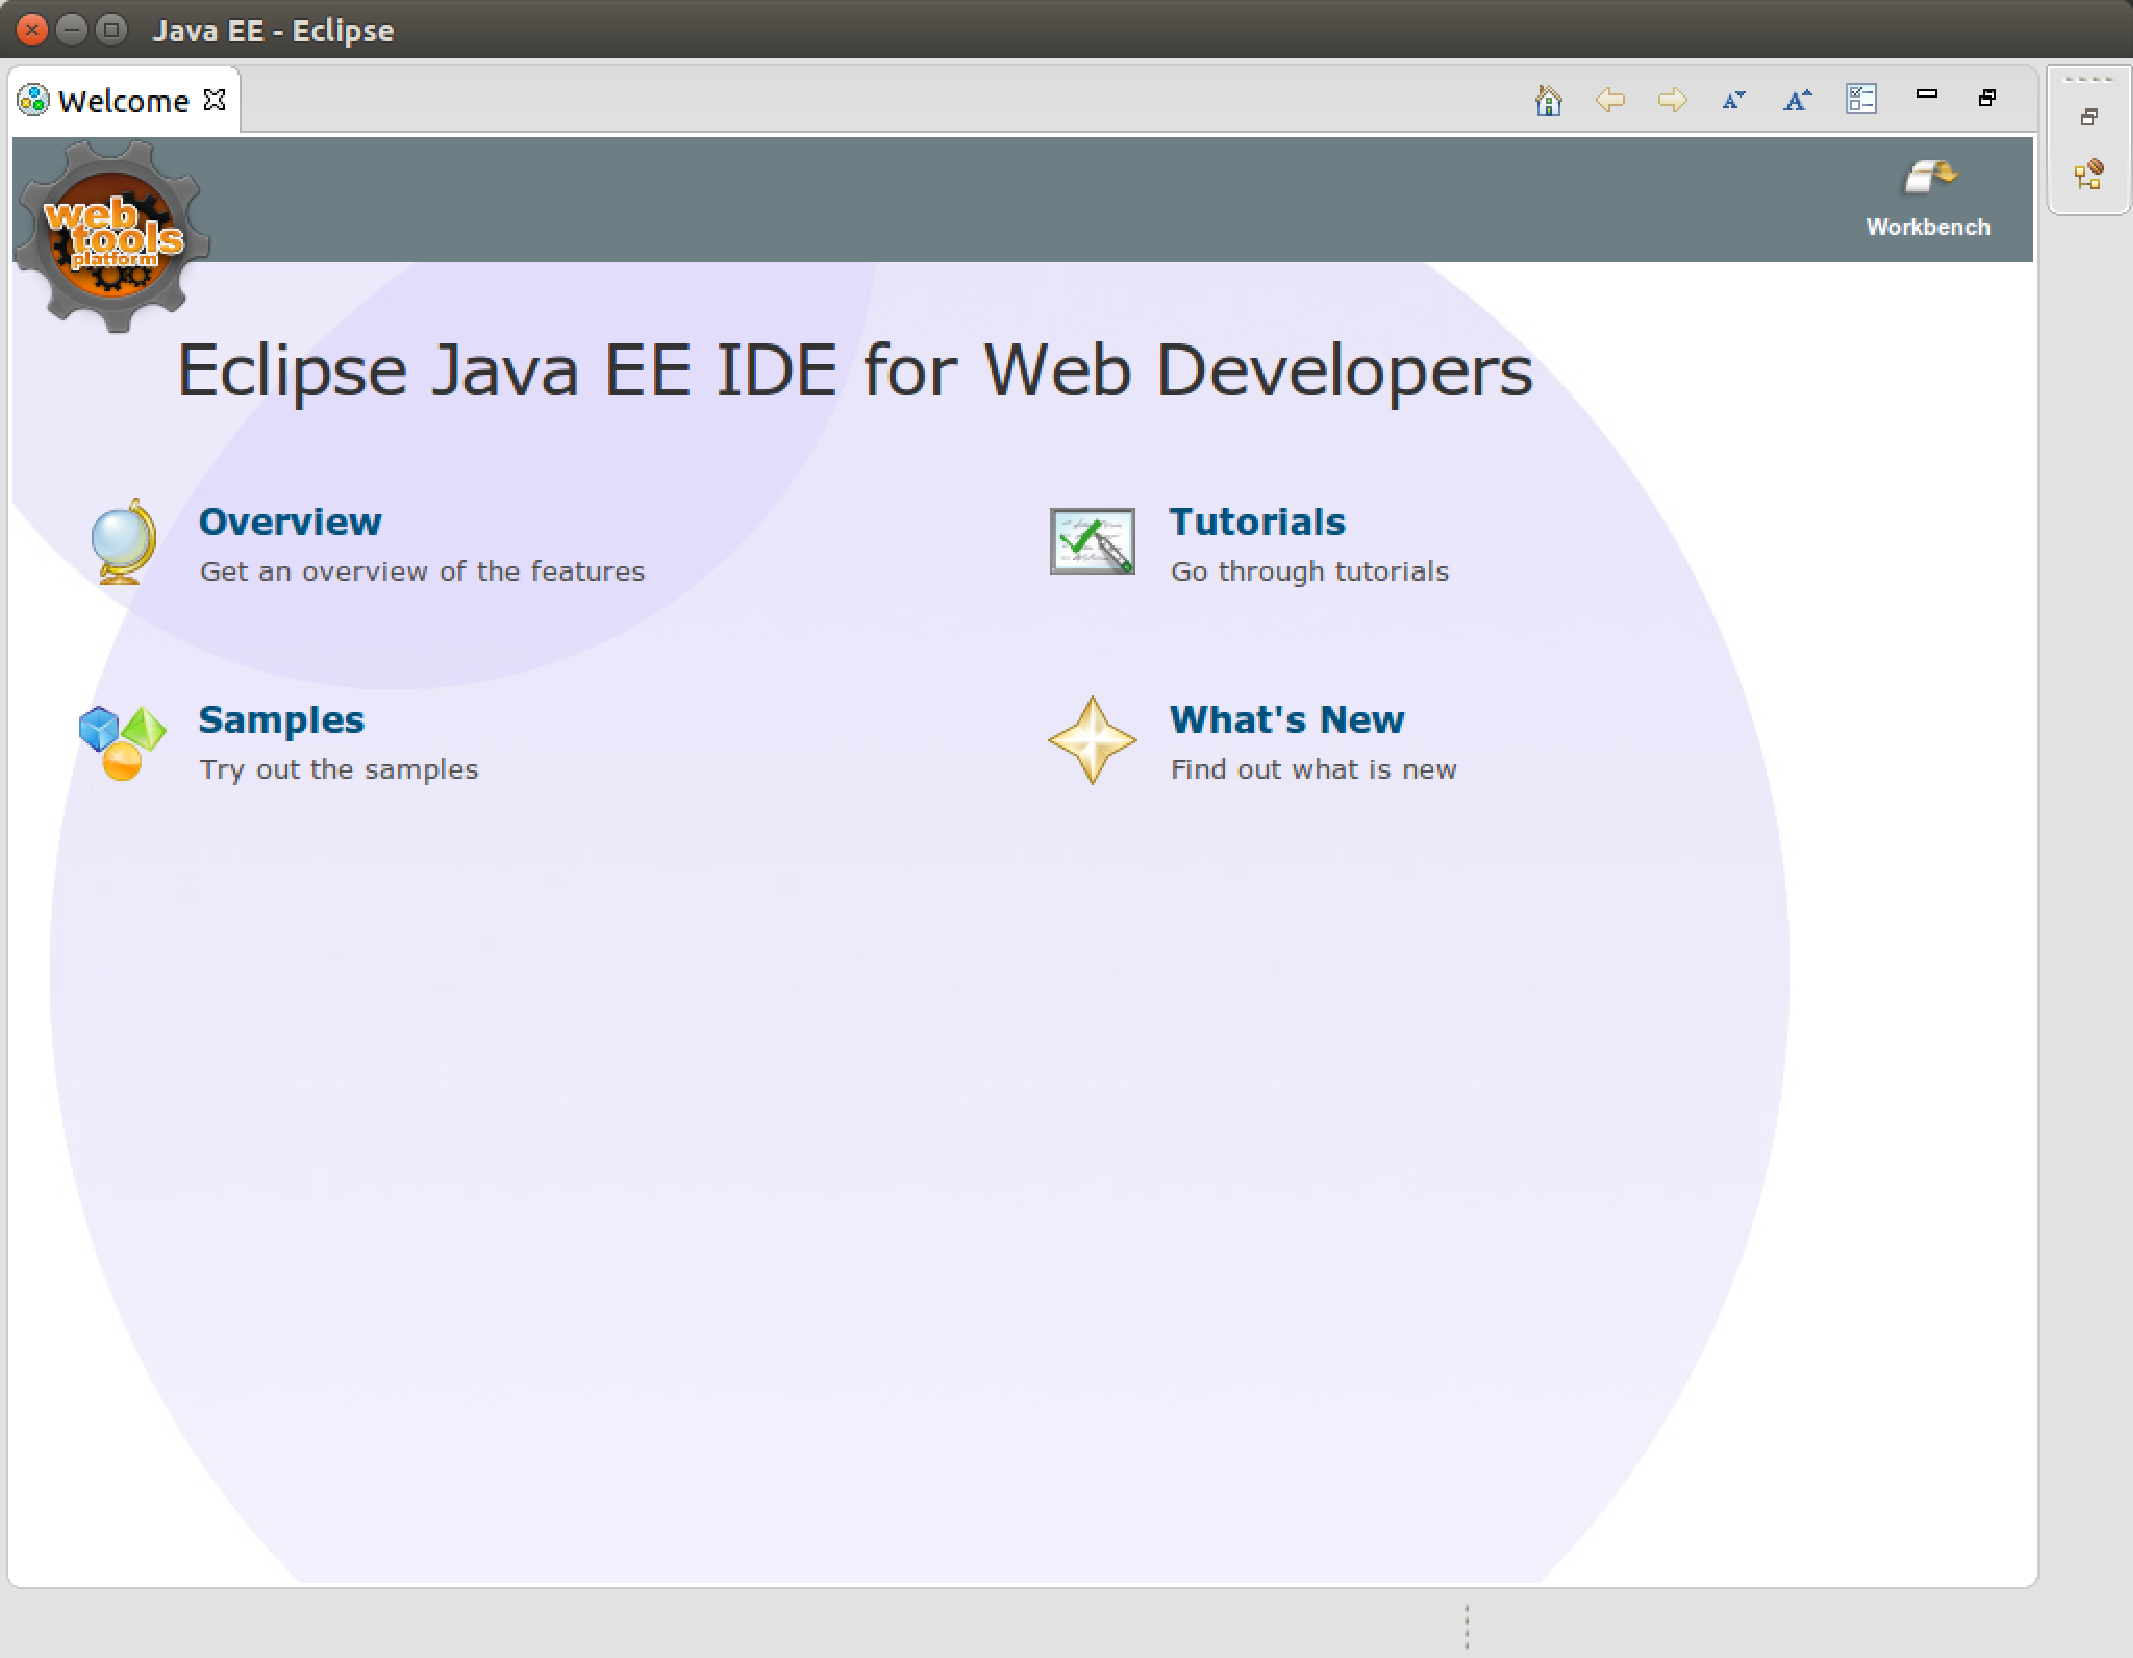
\includepdf[pages={1}]{img/eclipse/welcome.pdf}
}

% \pgfdeclareimage[height=\paperheight,width=\paperwidth]{start}{img/eclipse/start.png}
% \begin{frame}{Avvio di Eclipse}
%   \begin{center}
%     \pgfuseimage{start}
%   \end{center}
% \end{frame}
{
  \setbeamercolor{background canvas}{bg=}
  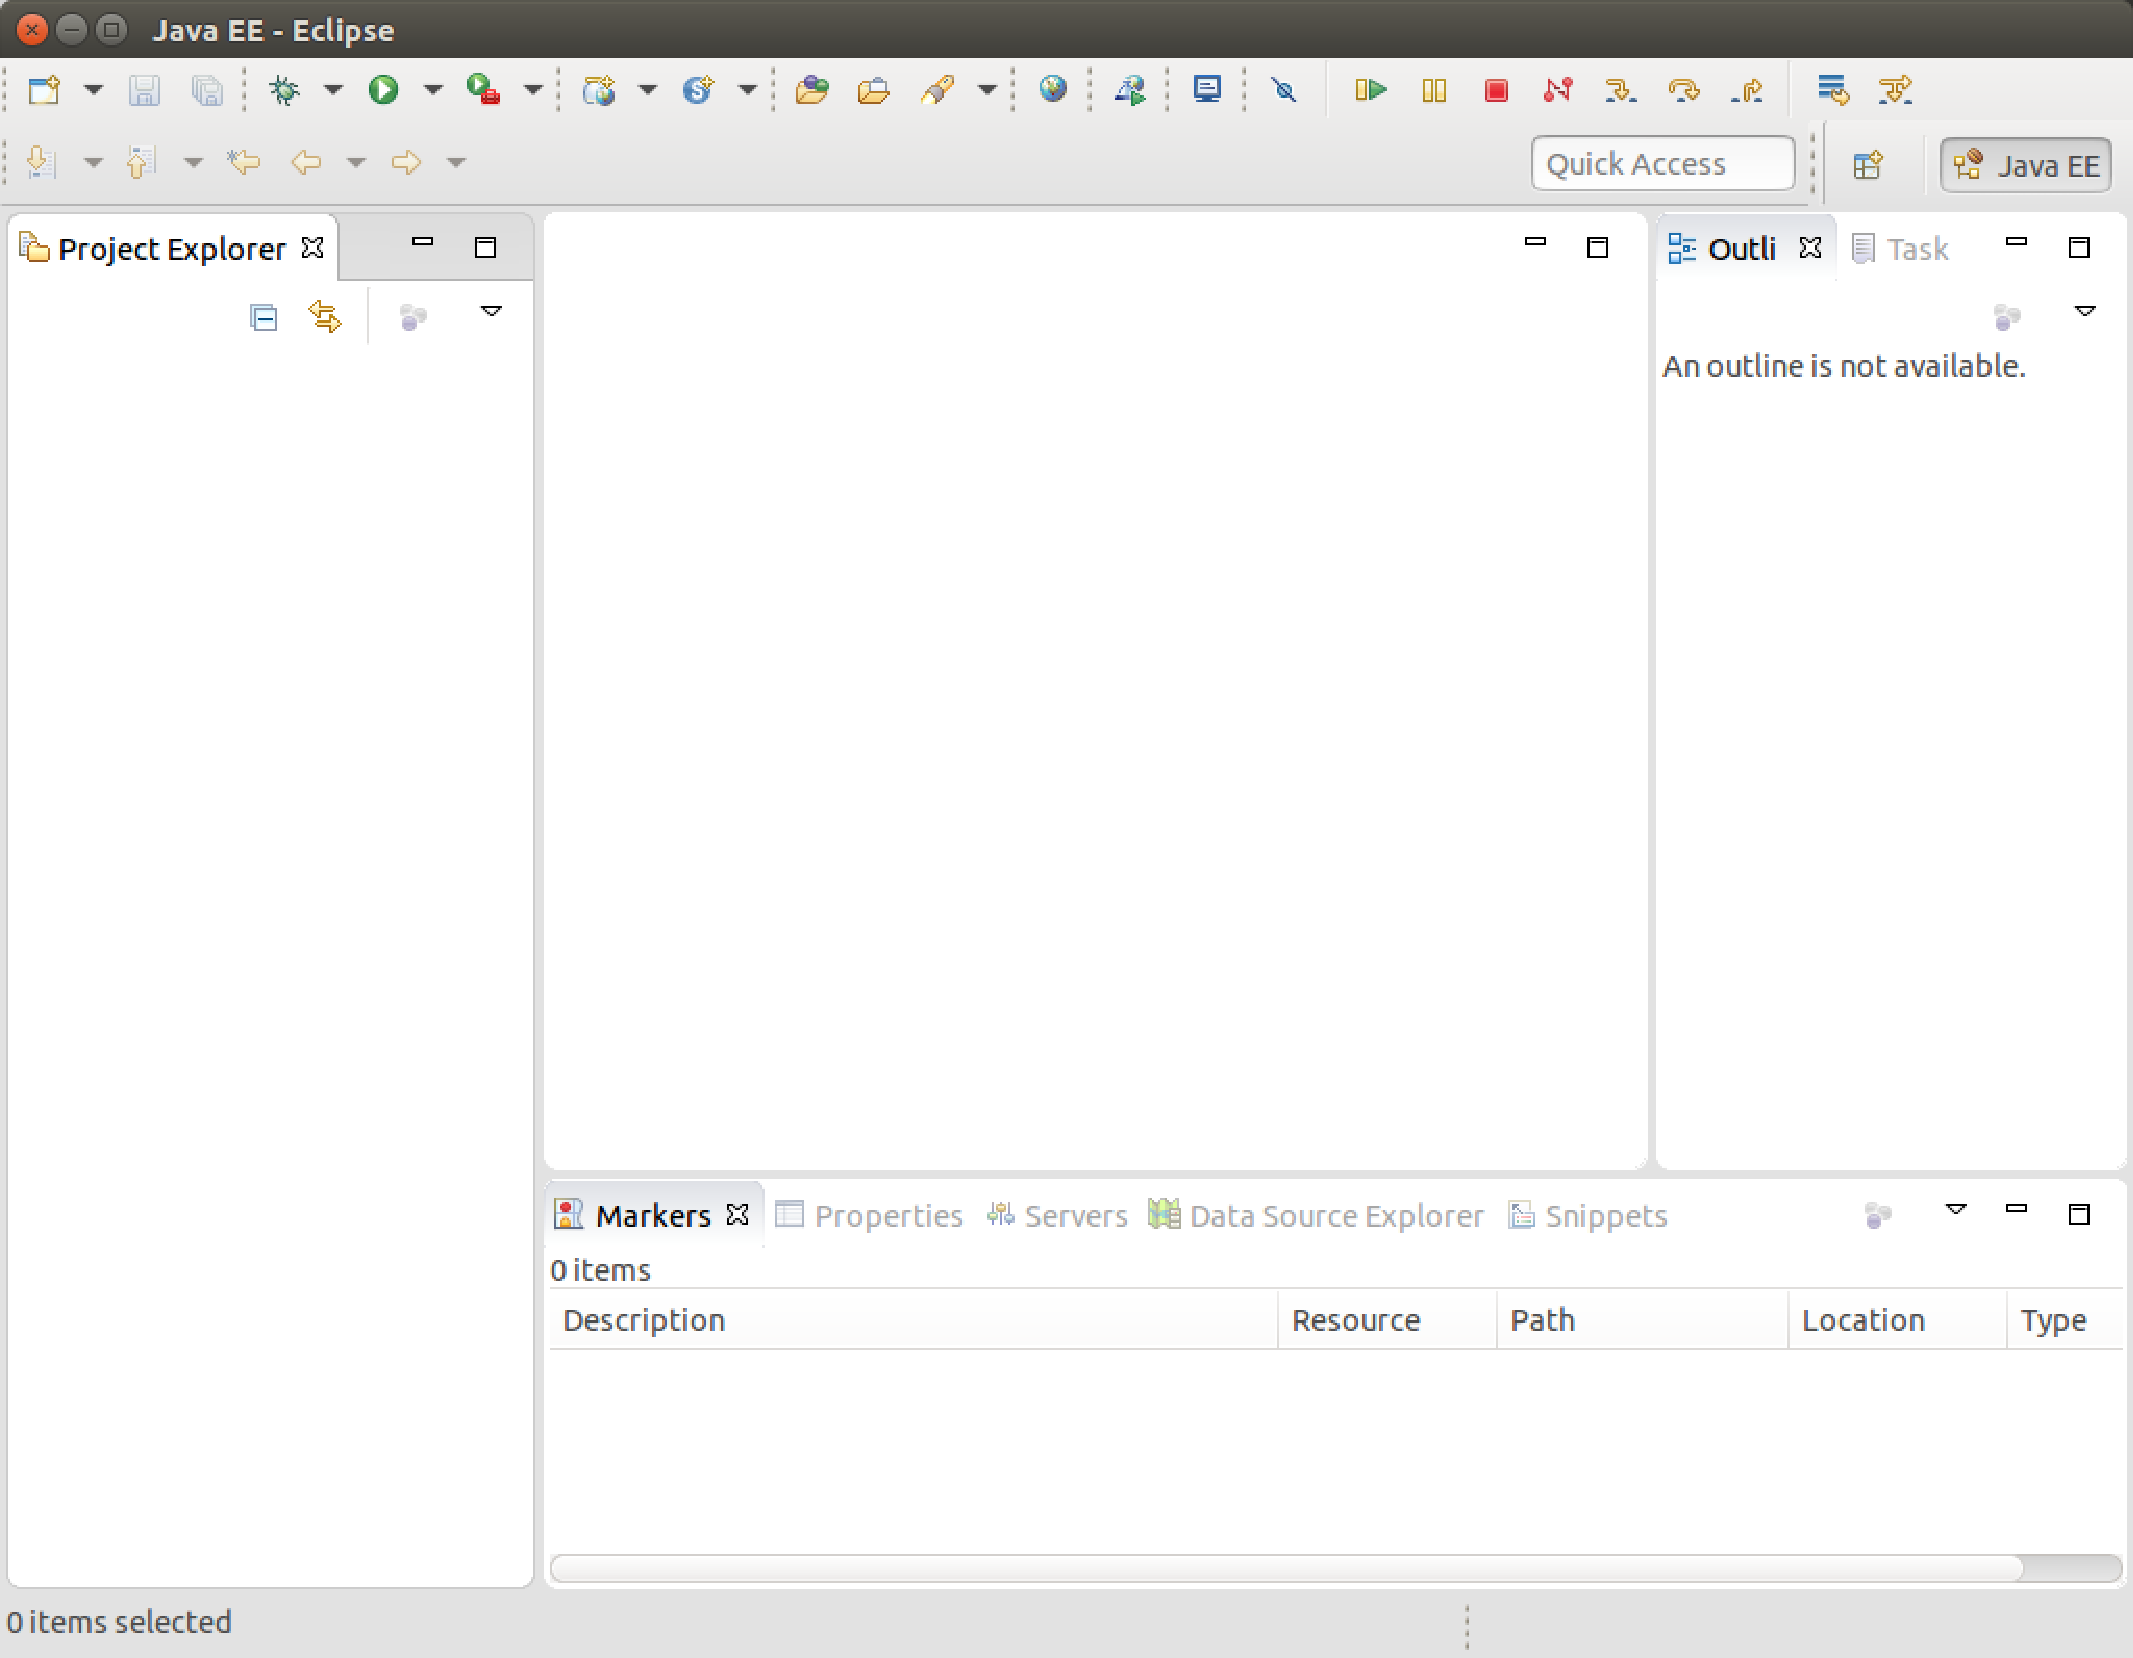
\includepdf[pages={1}]{img/eclipse/start.pdf}
}

% \pgfdeclareimage[height=\paperheight,width=\paperwidth]{new_project}{img/eclipse/new_project.png}
% \begin{frame}{Avvio di Eclipse}
%   \begin{center}
%     \pgfuseimage{new_project}
%   \end{center}
% \end{frame}
{
  \setbeamercolor{background canvas}{bg=}
  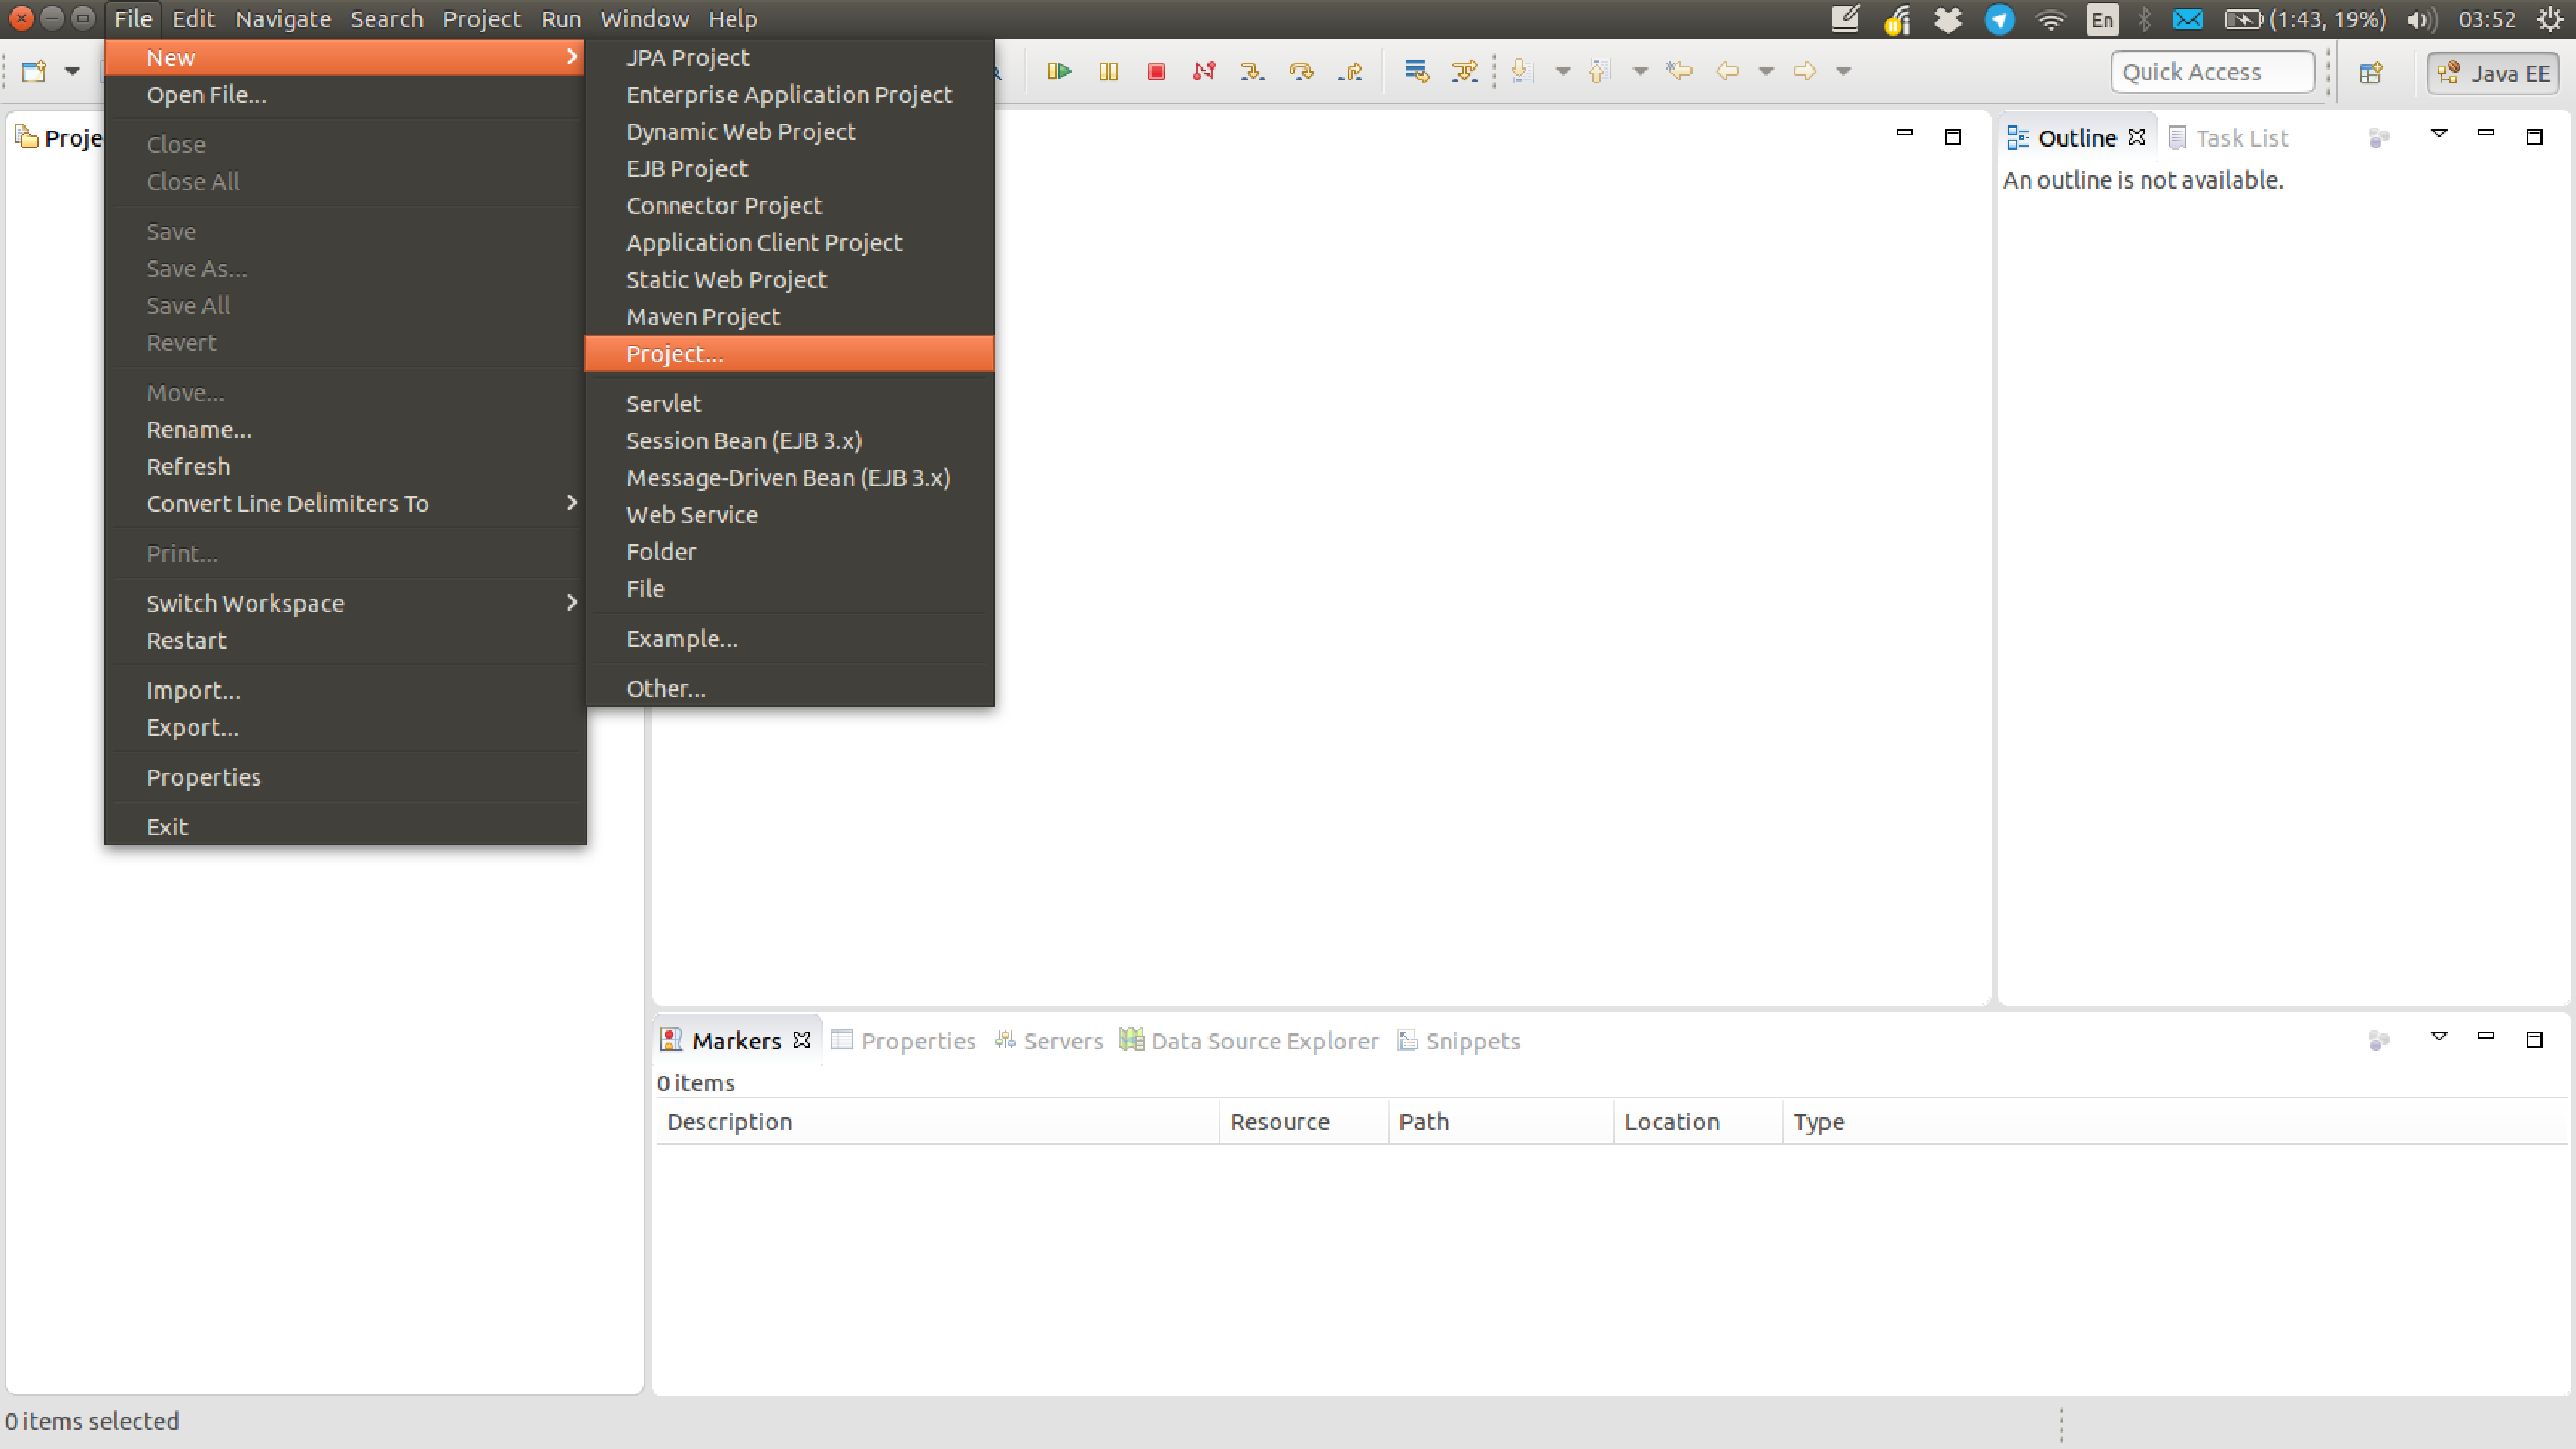
\includepdf[pages={1}]{img/eclipse/new_project.pdf}
}

% \pgfdeclareimage[height=\paperheight,width=\paperwidth]{new_java_project}{img/eclipse/new_java_project.png}
% \begin{frame}{Avvio di Eclipse}
%   \begin{center}
%     \pgfuseimage{new_java_project}
%   \end{center}
% \end{frame}
{
  \setbeamercolor{background canvas}{bg=}
  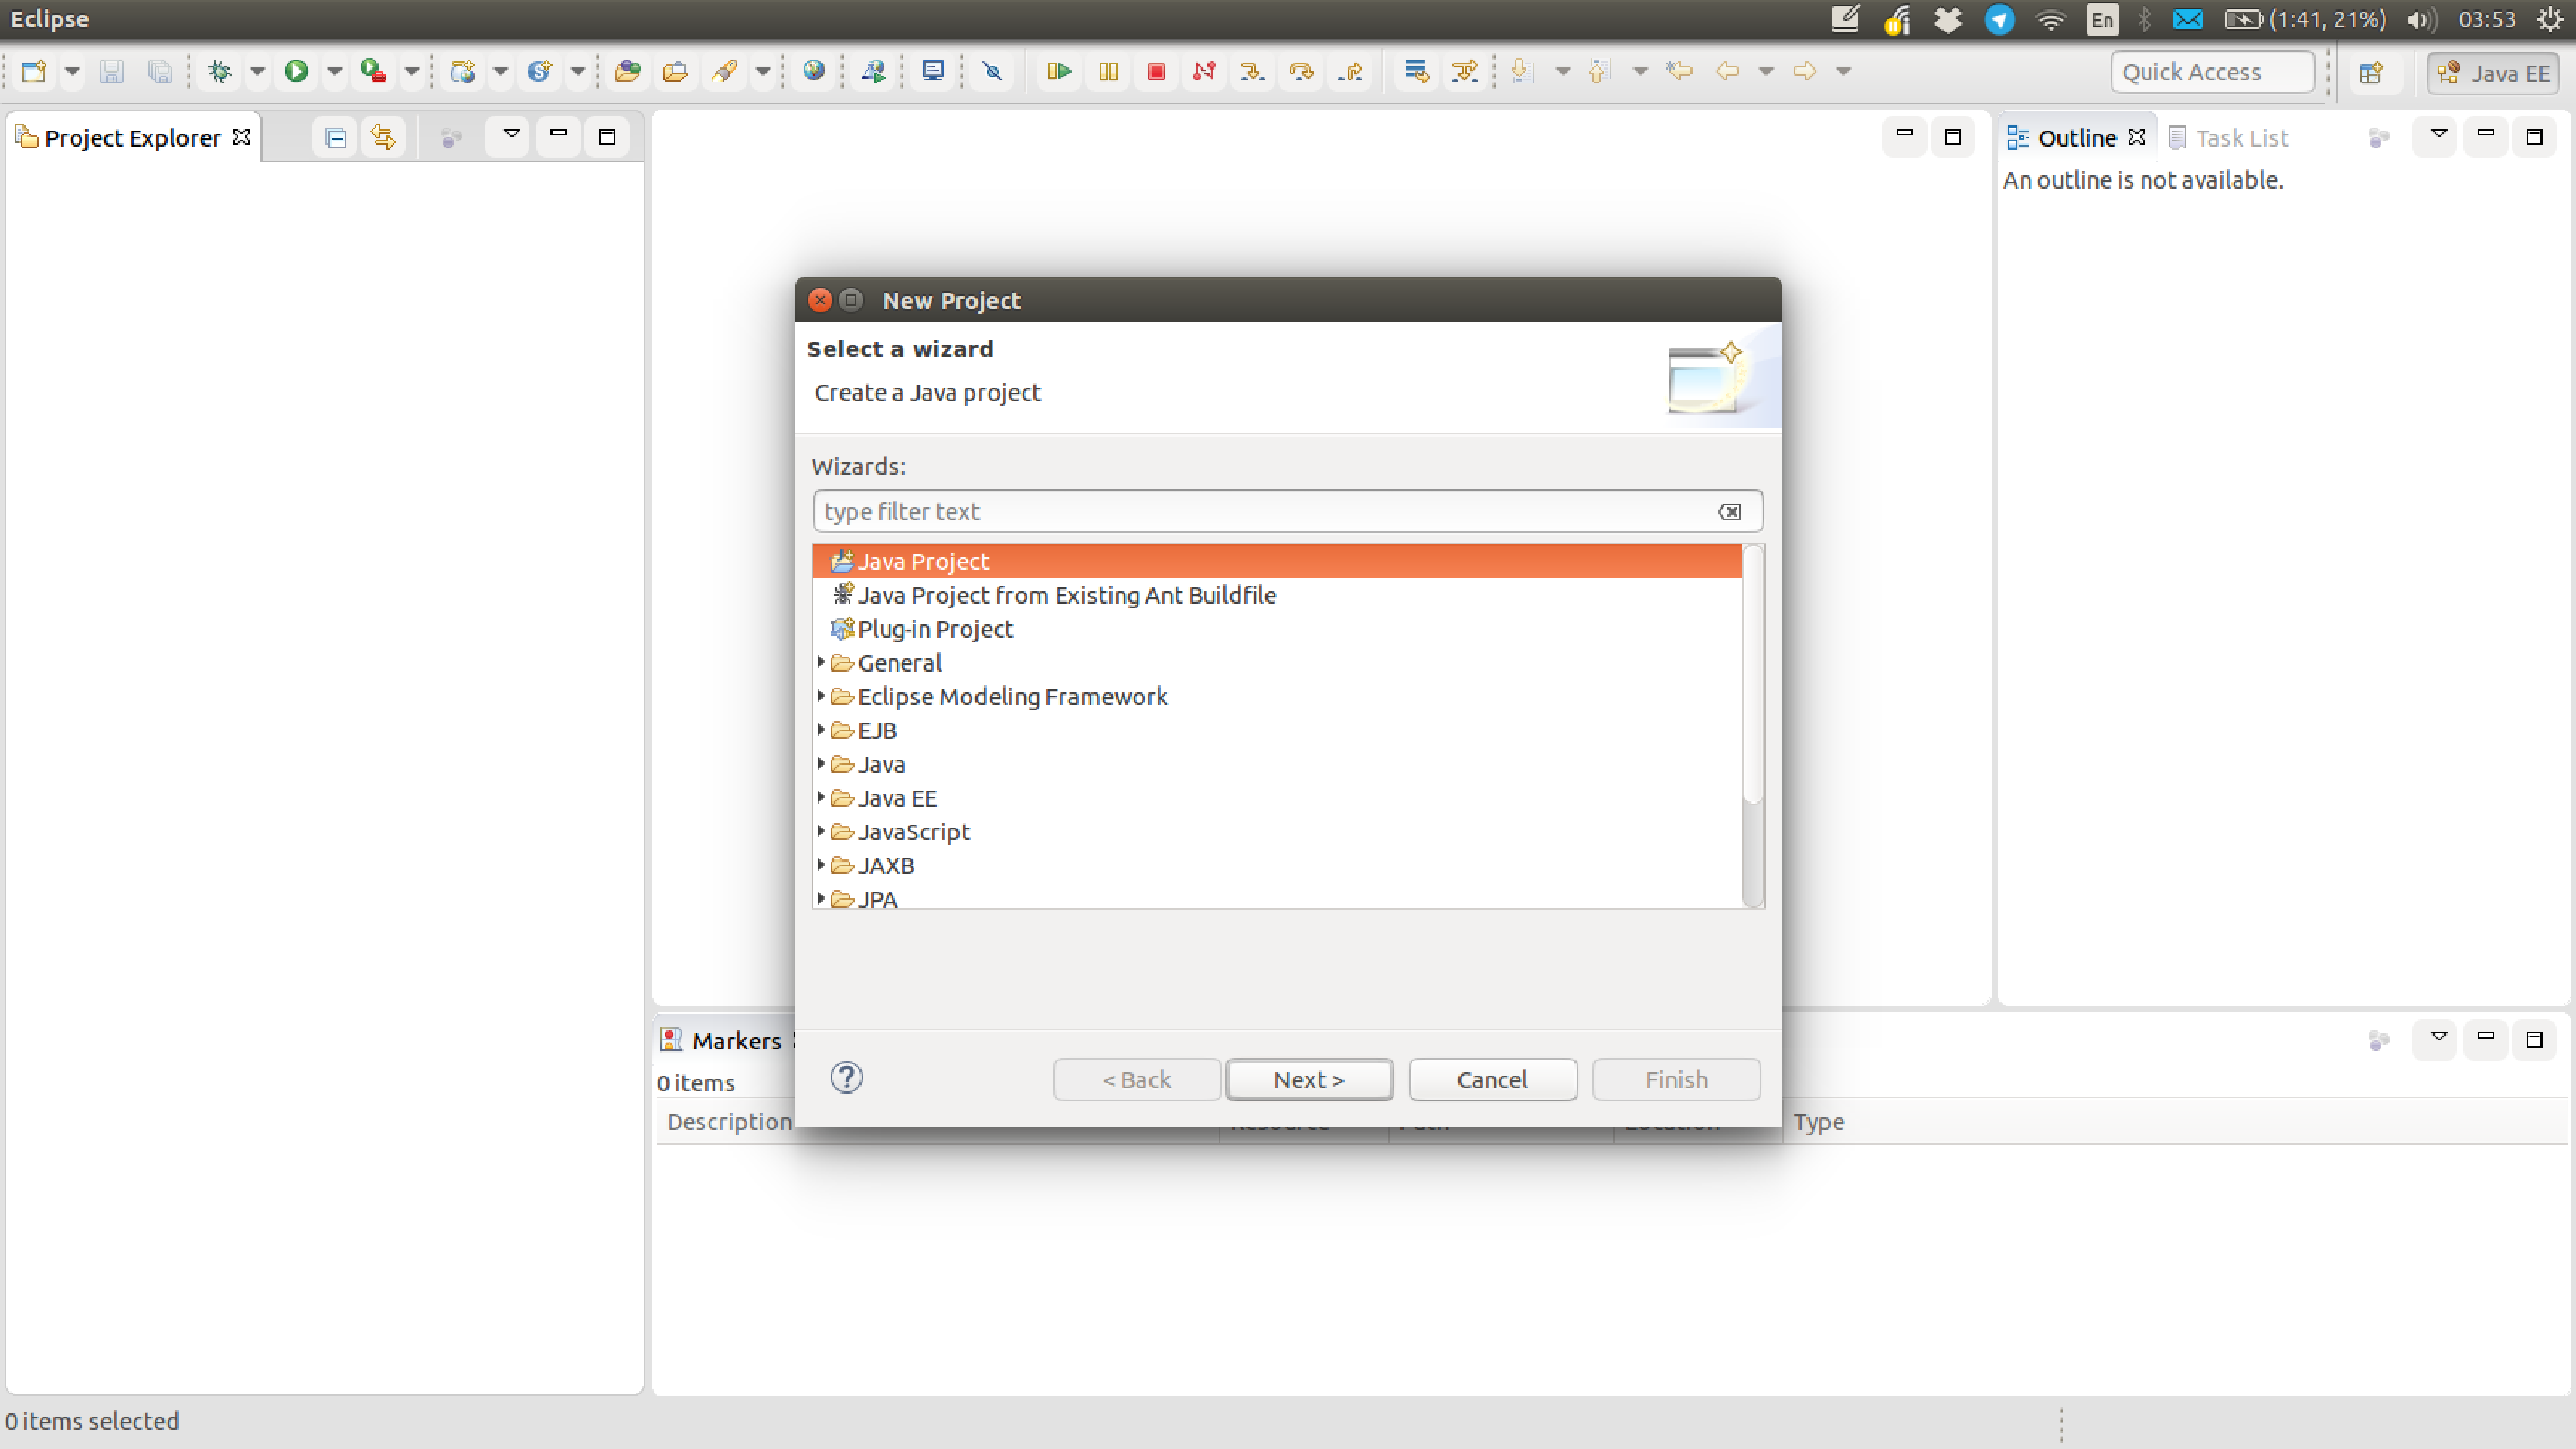
\includepdf[pages={1}]{img/eclipse/new_java_project.pdf}
}

% \pgfdeclareimage[height=\paperheight,width=\paperwidth]{create_project}{img/eclipse/create_project.png}
% \begin{frame}{Avvio di Eclipse}
%   \begin{center}
%     \pgfuseimage{create_project}
%   \end{center}
% \end{frame}
{
  \setbeamercolor{background canvas}{bg=}
  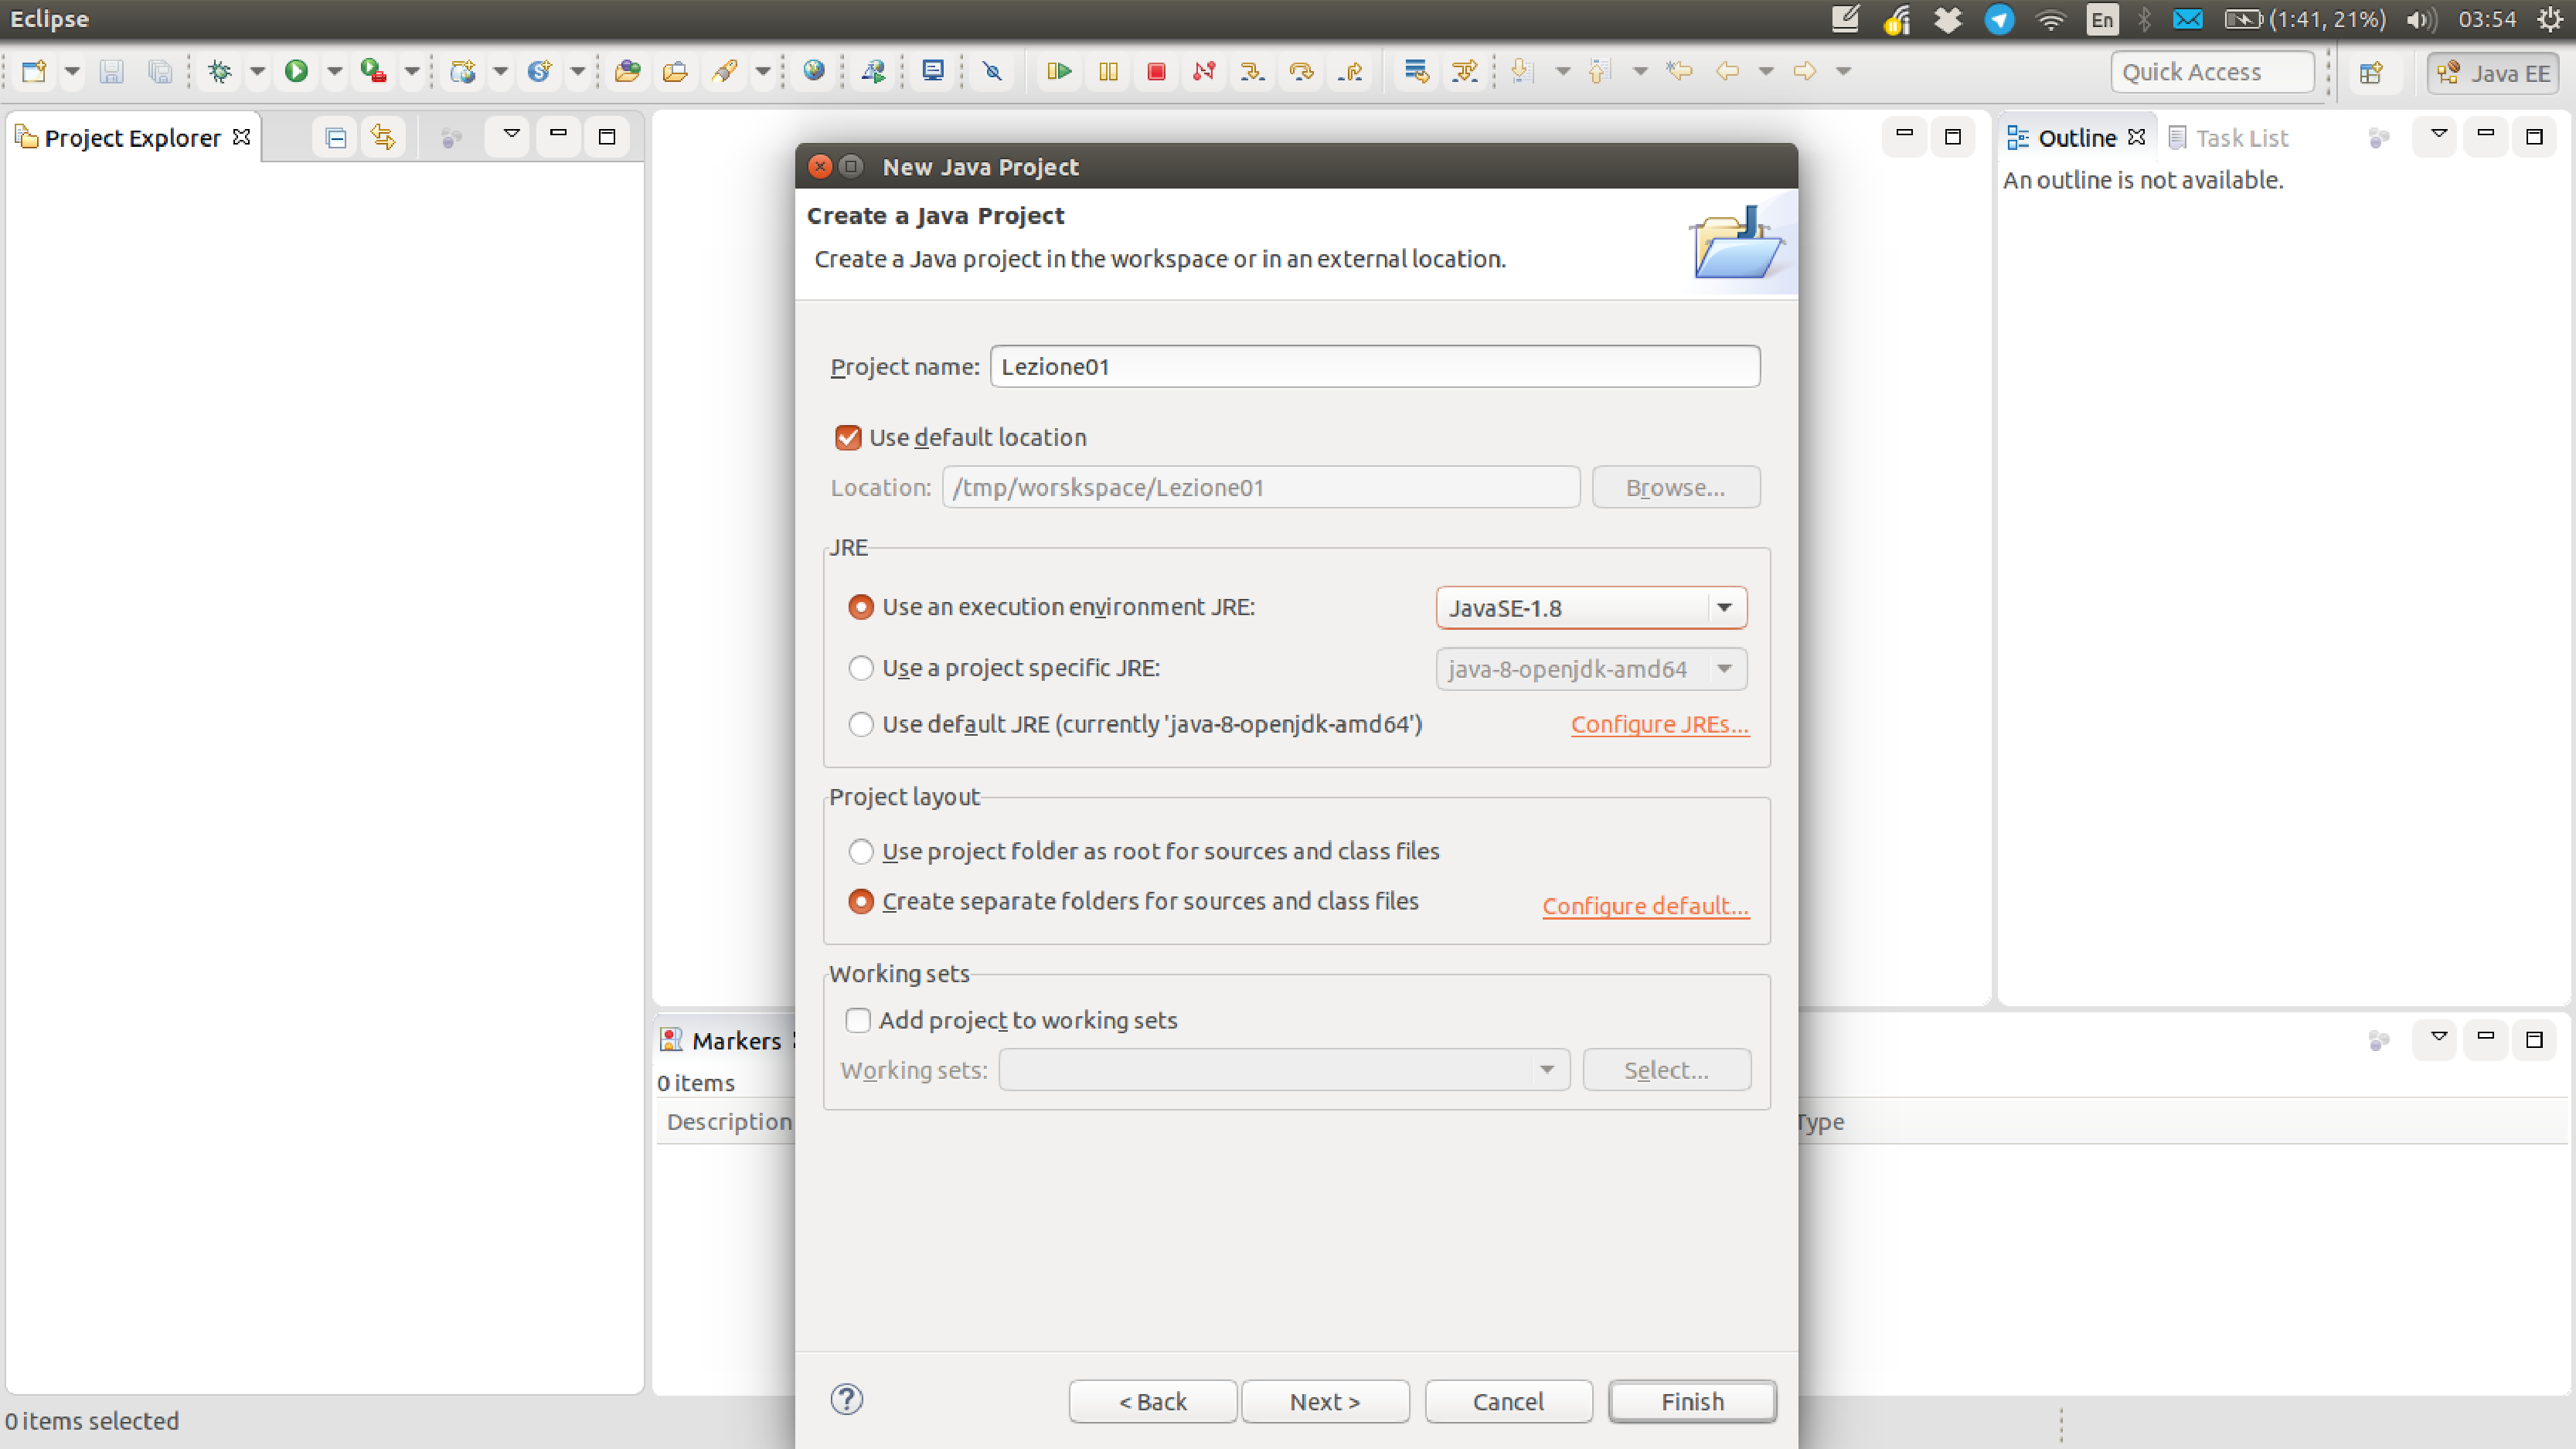
\includepdf[pages={1}]{img/eclipse/create_project.pdf}
}

% \pgfdeclareimage[height=\paperheight,width=\paperwidth]{project_created}{img/eclipse/project_created.png}
% \begin{frame}{Avvio di Eclipse}
%   \begin{center}
%     \pgfuseimage{project_created}
%   \end{center}
% \end{frame}
{
  \setbeamercolor{background canvas}{bg=}
  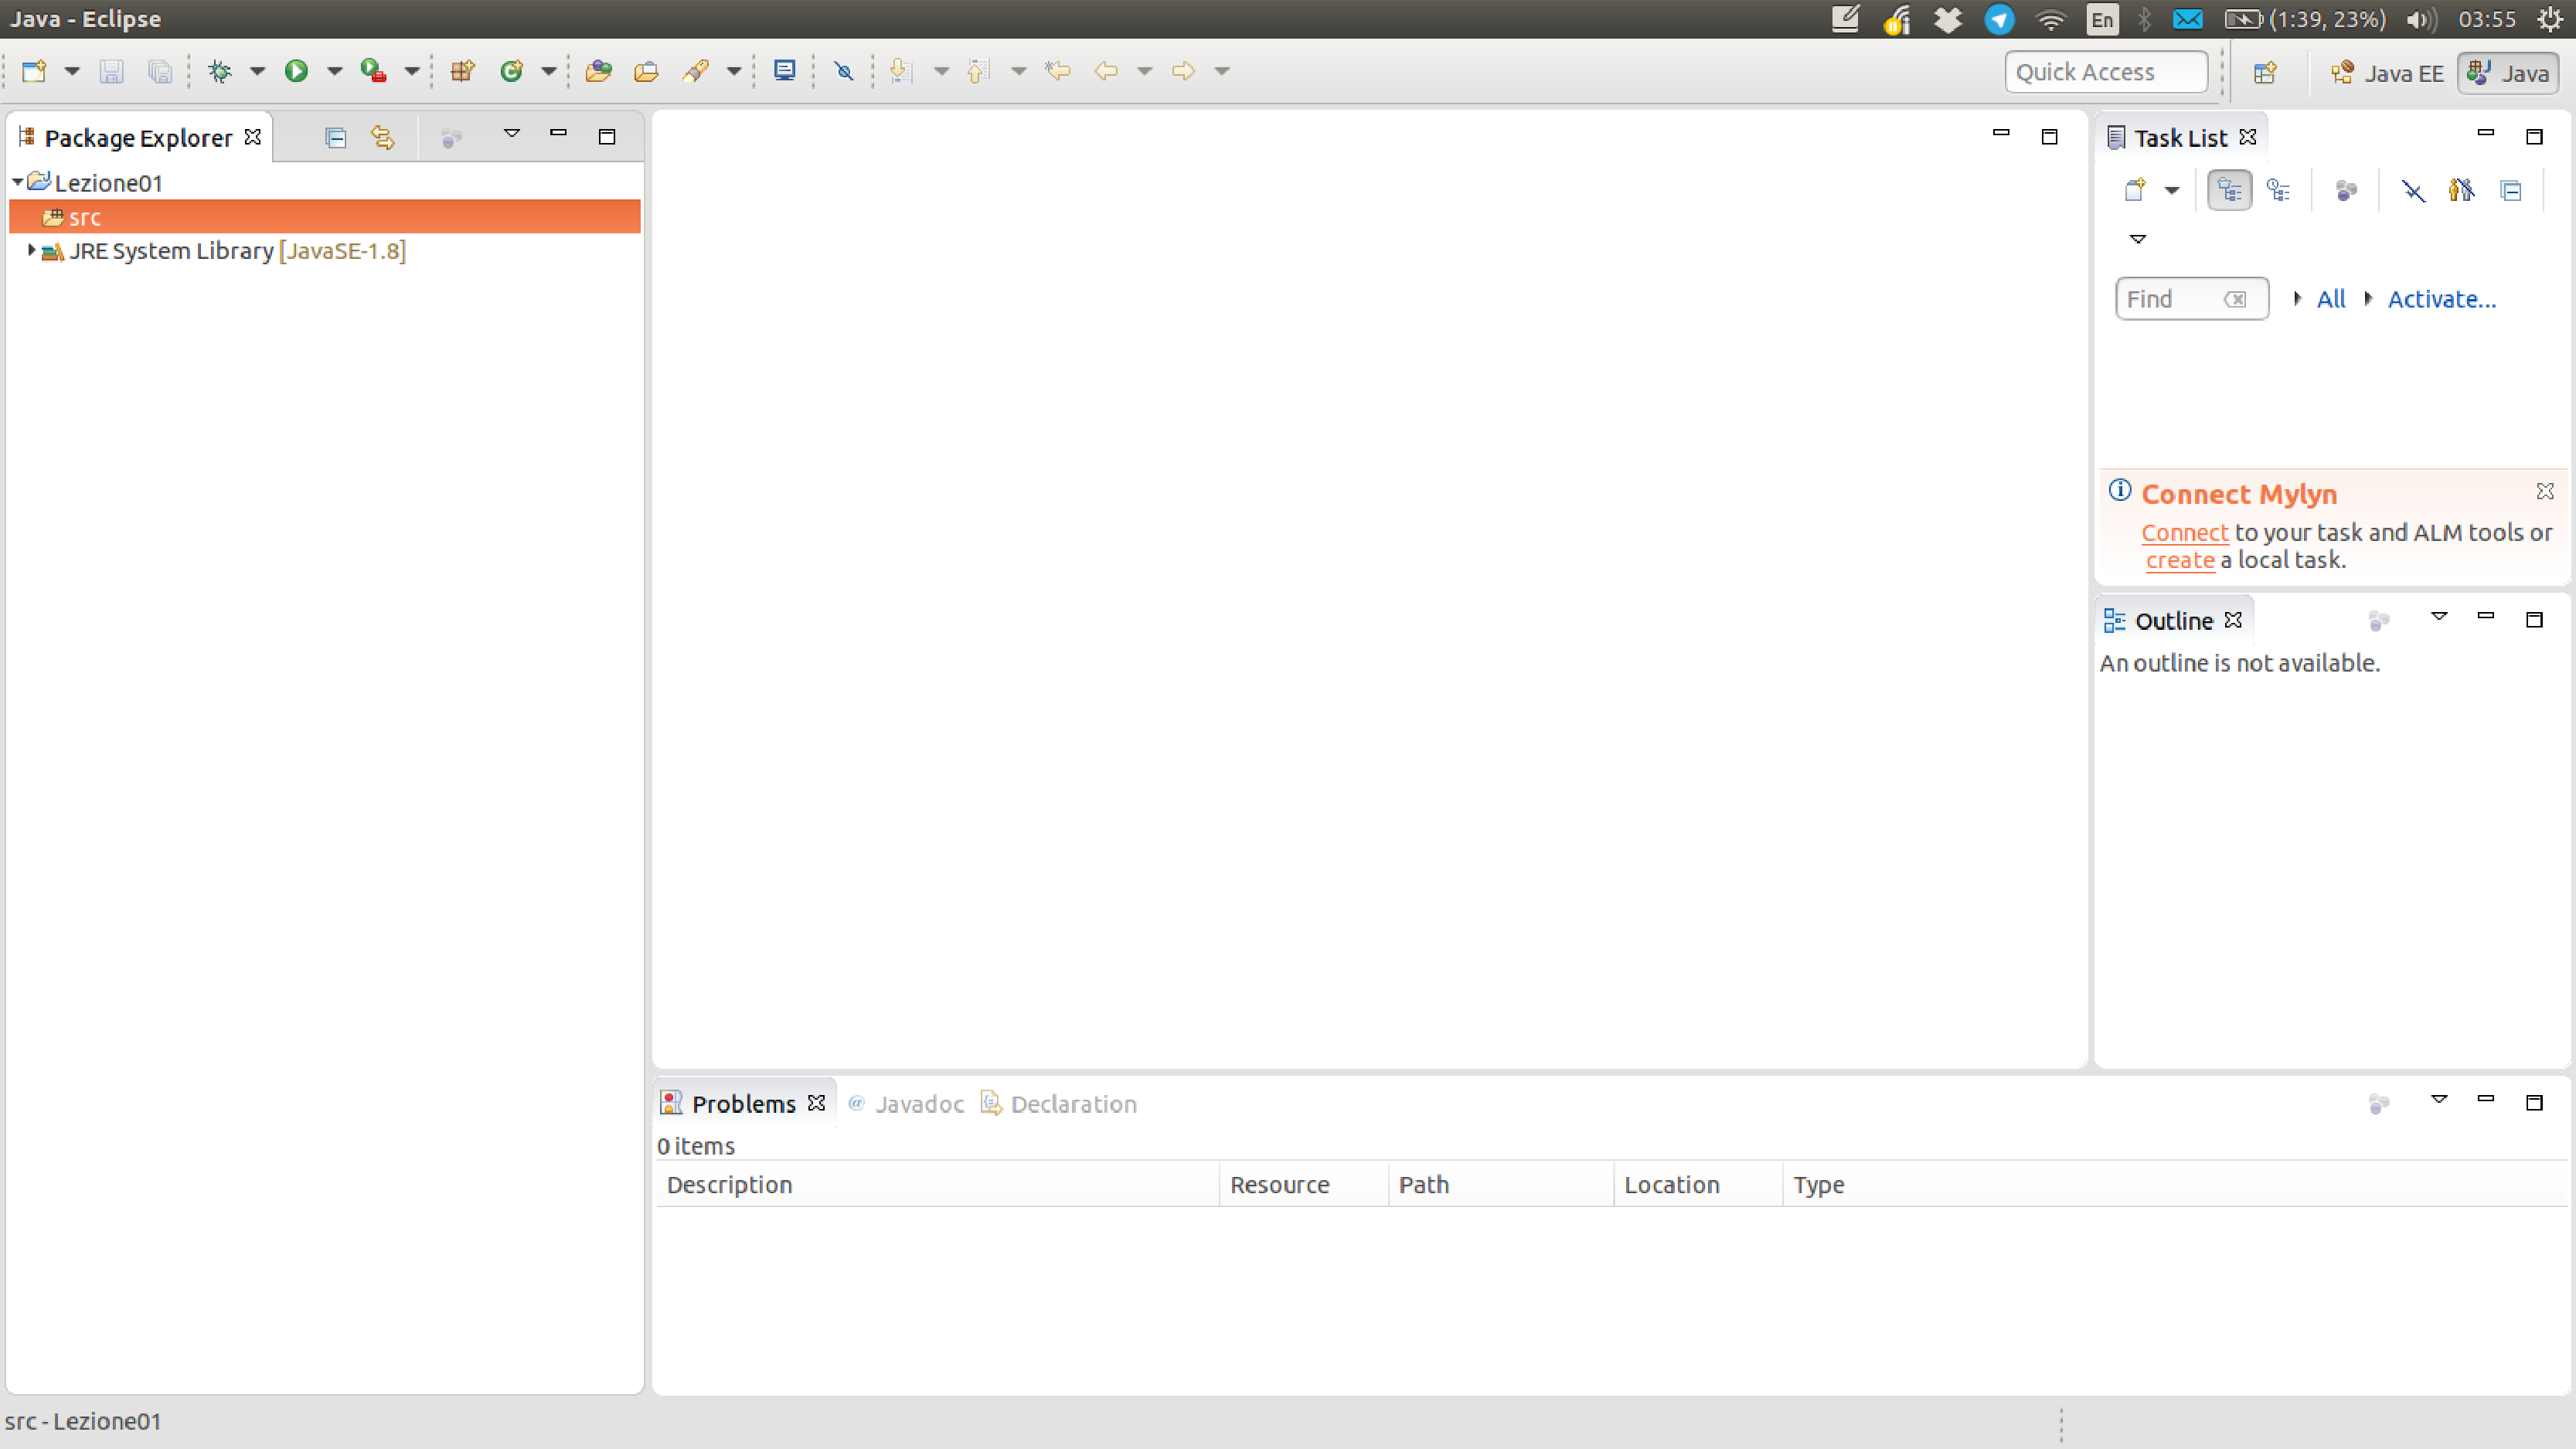
\includepdf[pages={1}]{img/eclipse/project_created.pdf}
}

% \pgfdeclareimage[height=\paperheight,width=\paperwidth]{new_class}{img/eclipse/new_class.png}
% \begin{frame}{Avvio di Eclipse}
%   \begin{center}
%     \pgfuseimage{new_class}
%   \end{center}
% \end{frame}
{
  \setbeamercolor{background canvas}{bg=}
  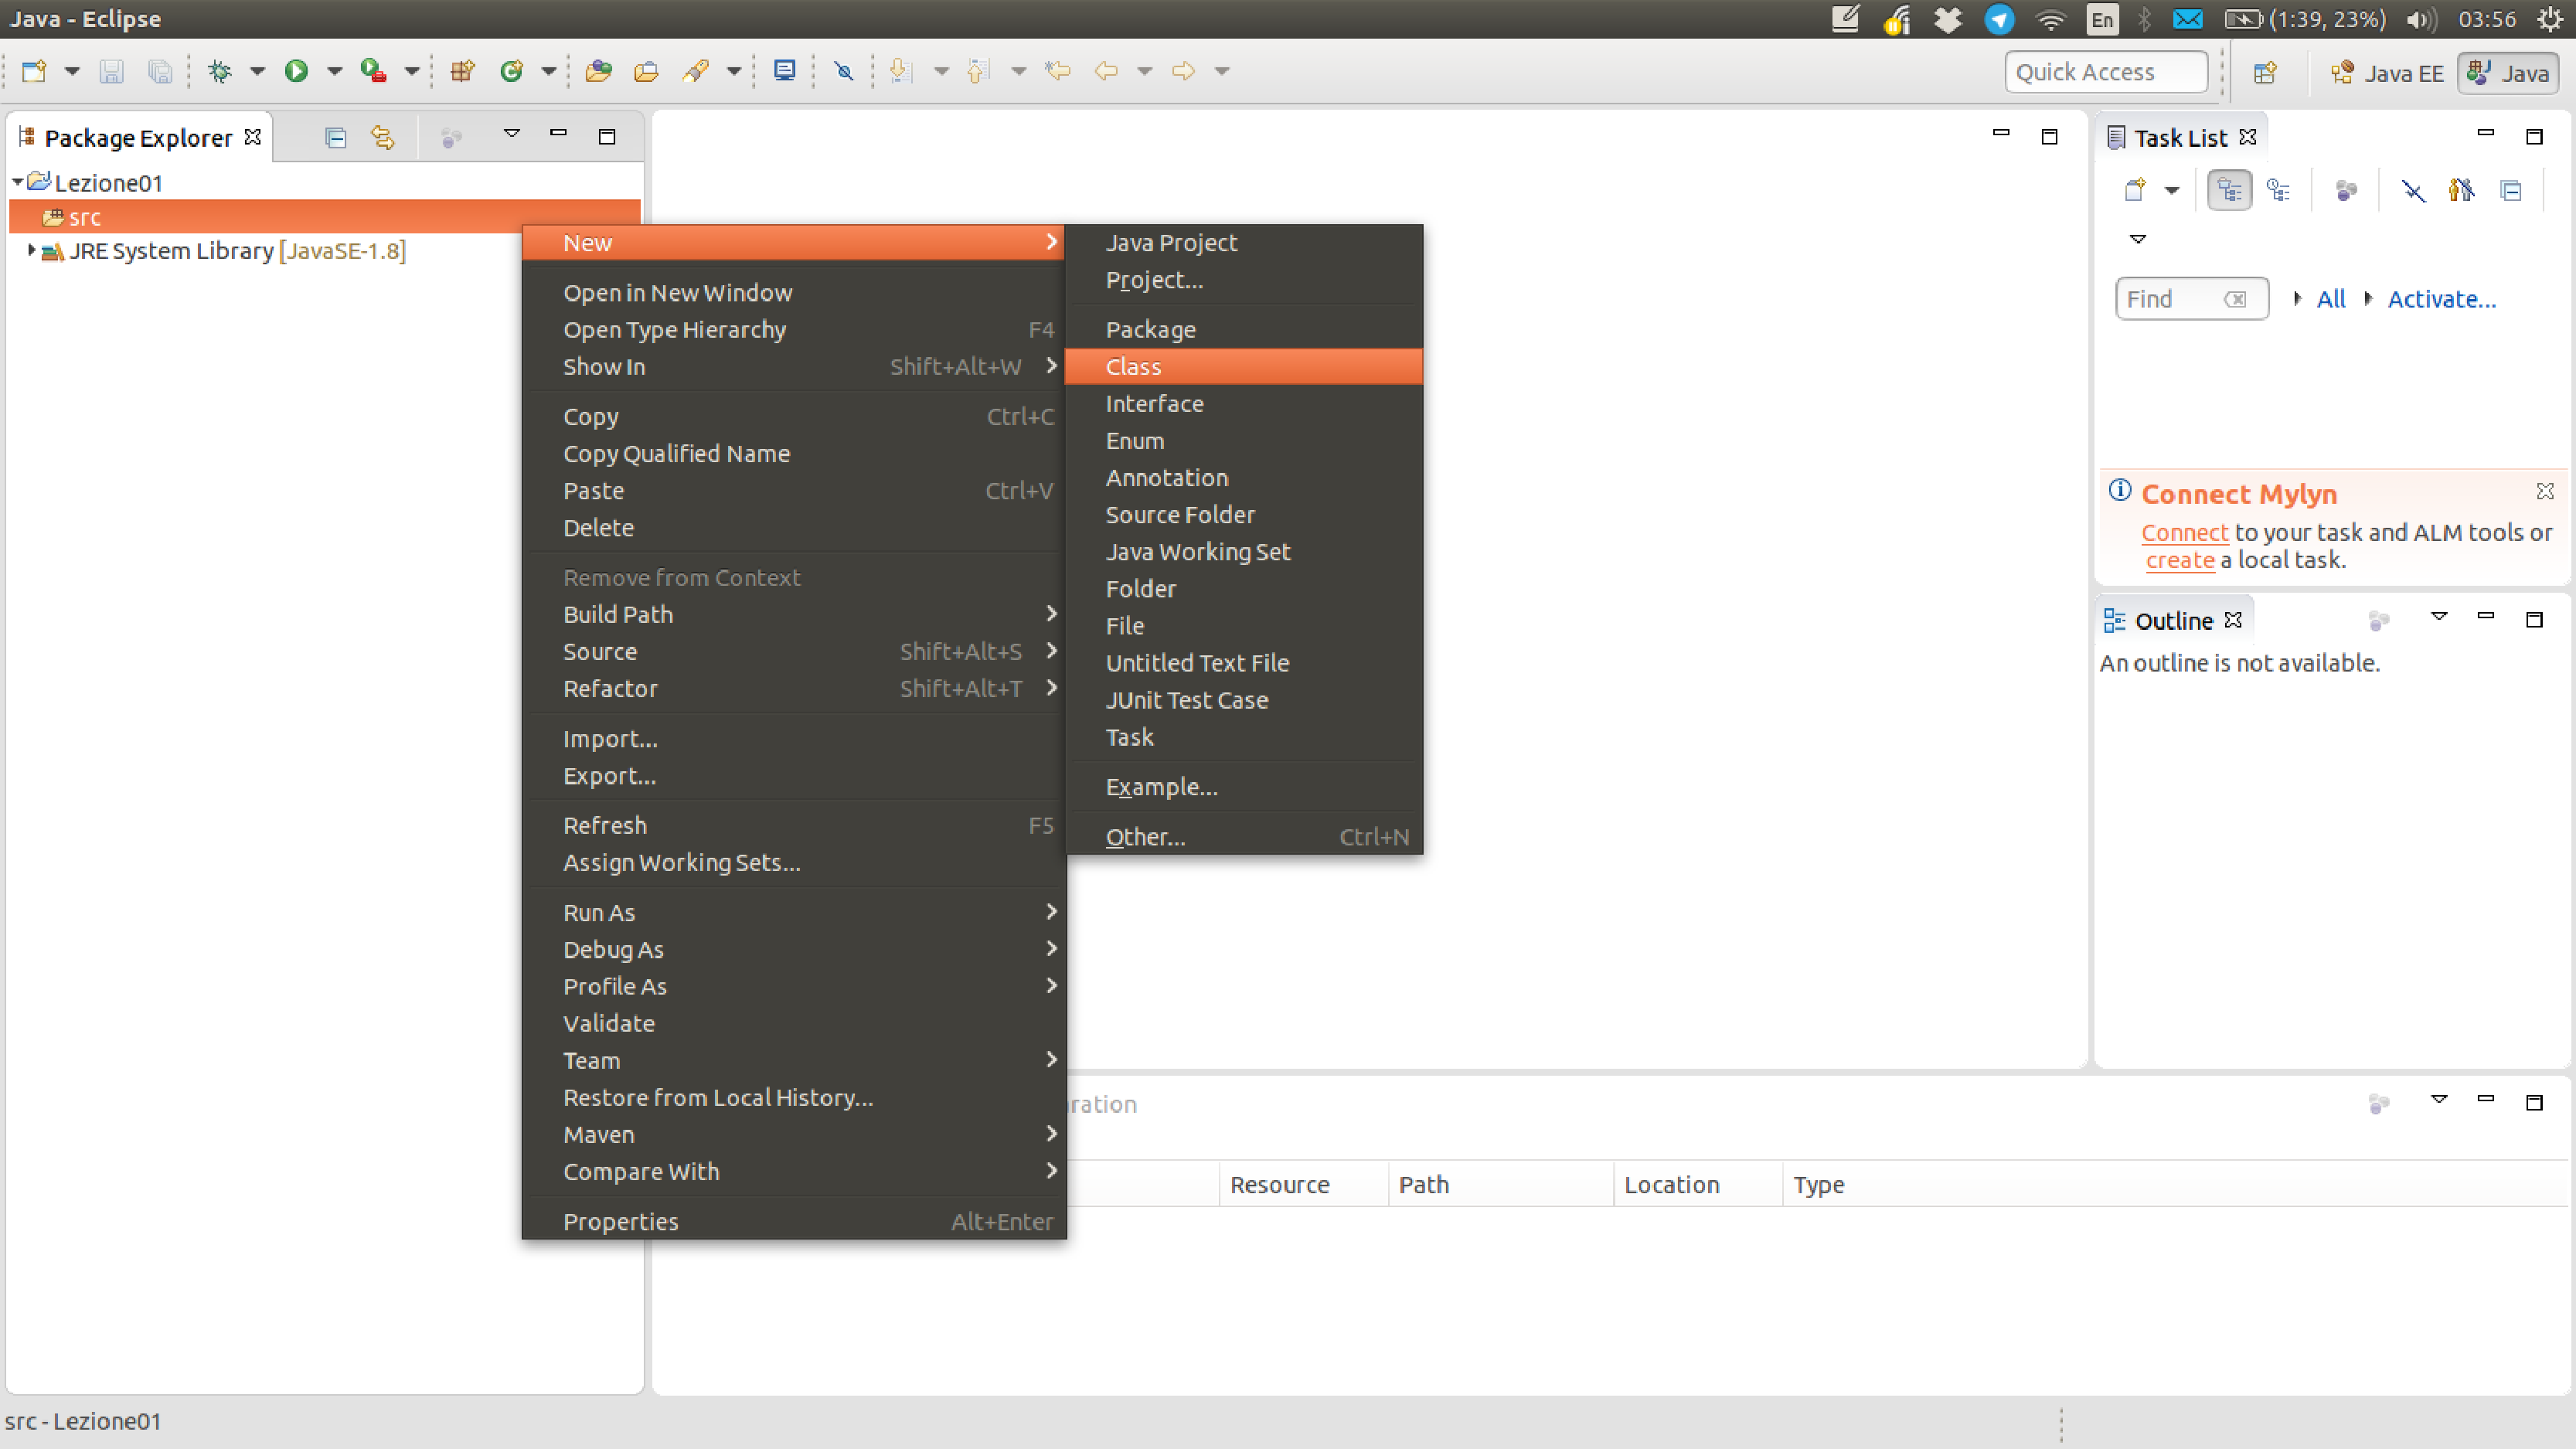
\includepdf[pages={1}]{img/eclipse/new_class.pdf}
}

% \pgfdeclareimage[height=\paperheight,width=\paperwidth]{create_class}{img/eclipse/create_class.png}
% \begin{frame}{Avvio di Eclipse}
%   \begin{center}
%     \pgfuseimage{create_class}
%   \end{center}
% \end{frame}
{
  \setbeamercolor{background canvas}{bg=}
  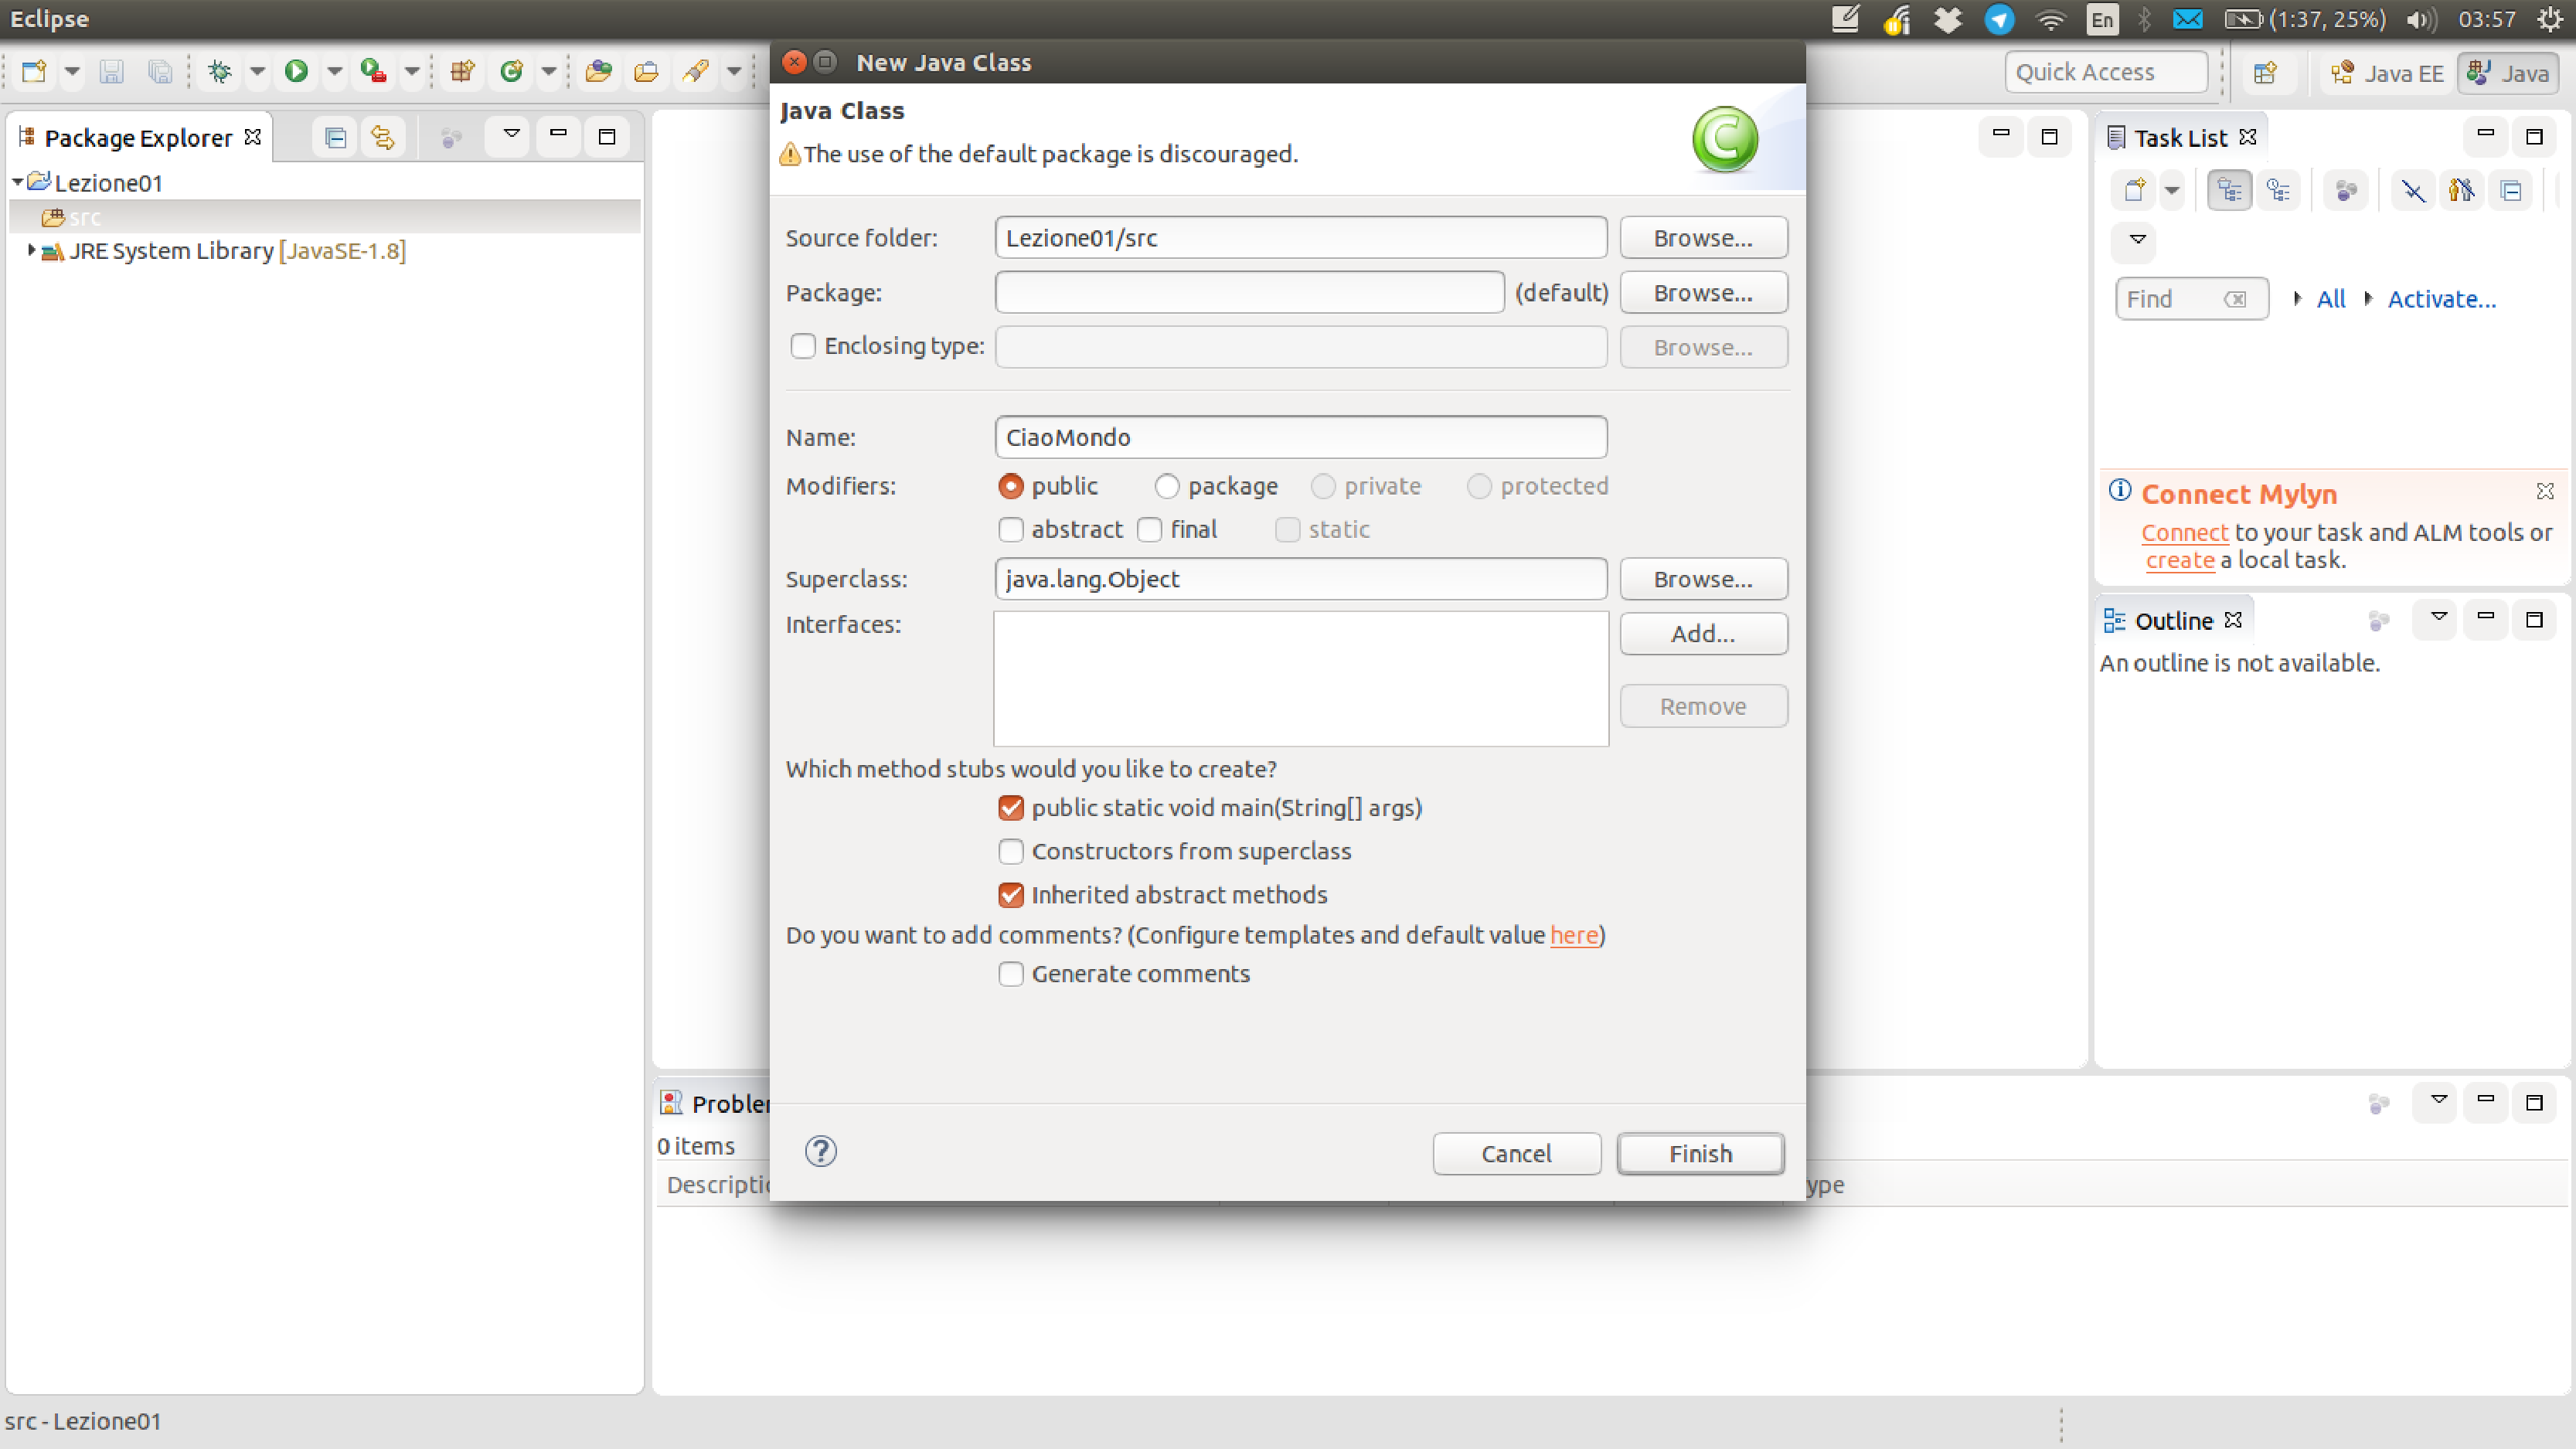
\includepdf[pages={1}]{img/eclipse/create_class.pdf}
}

% \pgfdeclareimage[height=\paperheight,width=\paperwidth]{class_created}{img/eclipse/class_created.png}
% \begin{frame}{Avvio di Eclipse}
%   \begin{center}
%     \pgfuseimage{class_created}
%   \end{center}
% \end{frame}
{
  \setbeamercolor{background canvas}{bg=}
  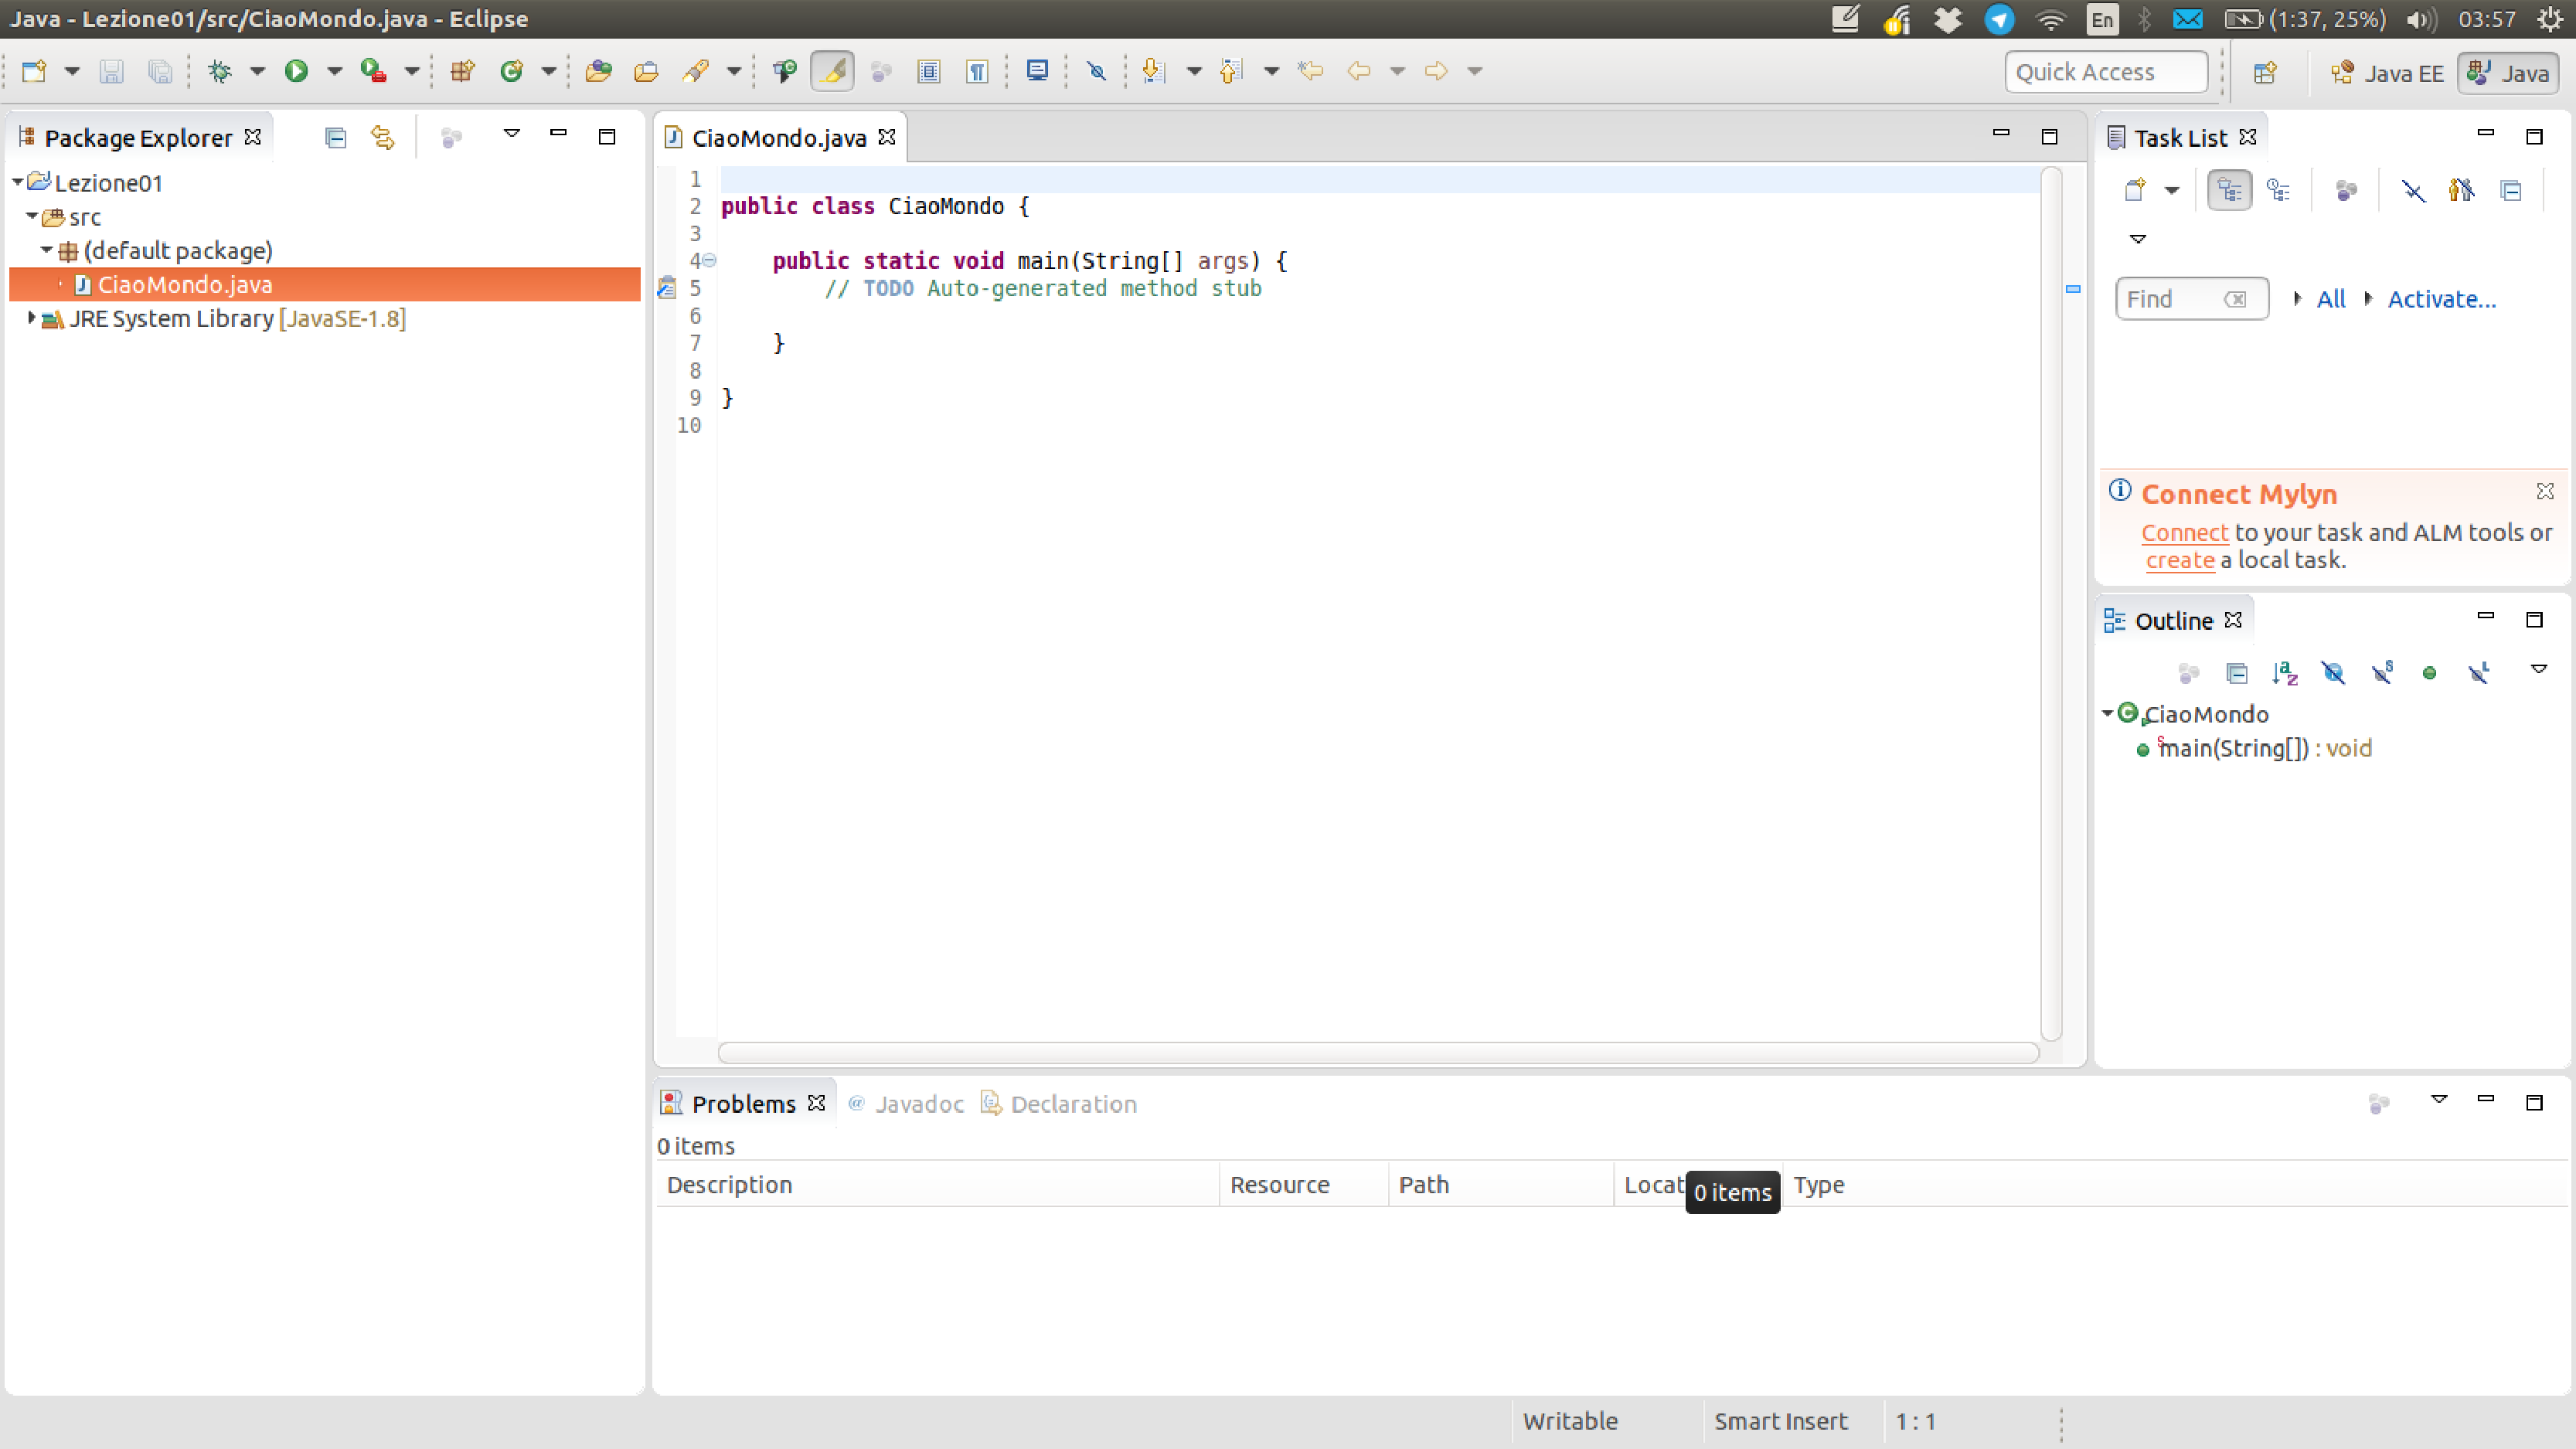
\includepdf[pages={1}]{img/eclipse/class_created.pdf}
}

% \pgfdeclareimage[height=\paperheight,width=\paperwidth]{code}{img/eclipse/code.png}
% \begin{frame}{Avvio di Eclipse}
%   \begin{center}
%     \pgfuseimage{code}
%   \end{center}
% \end{frame}
{
  \setbeamercolor{background canvas}{bg=}
  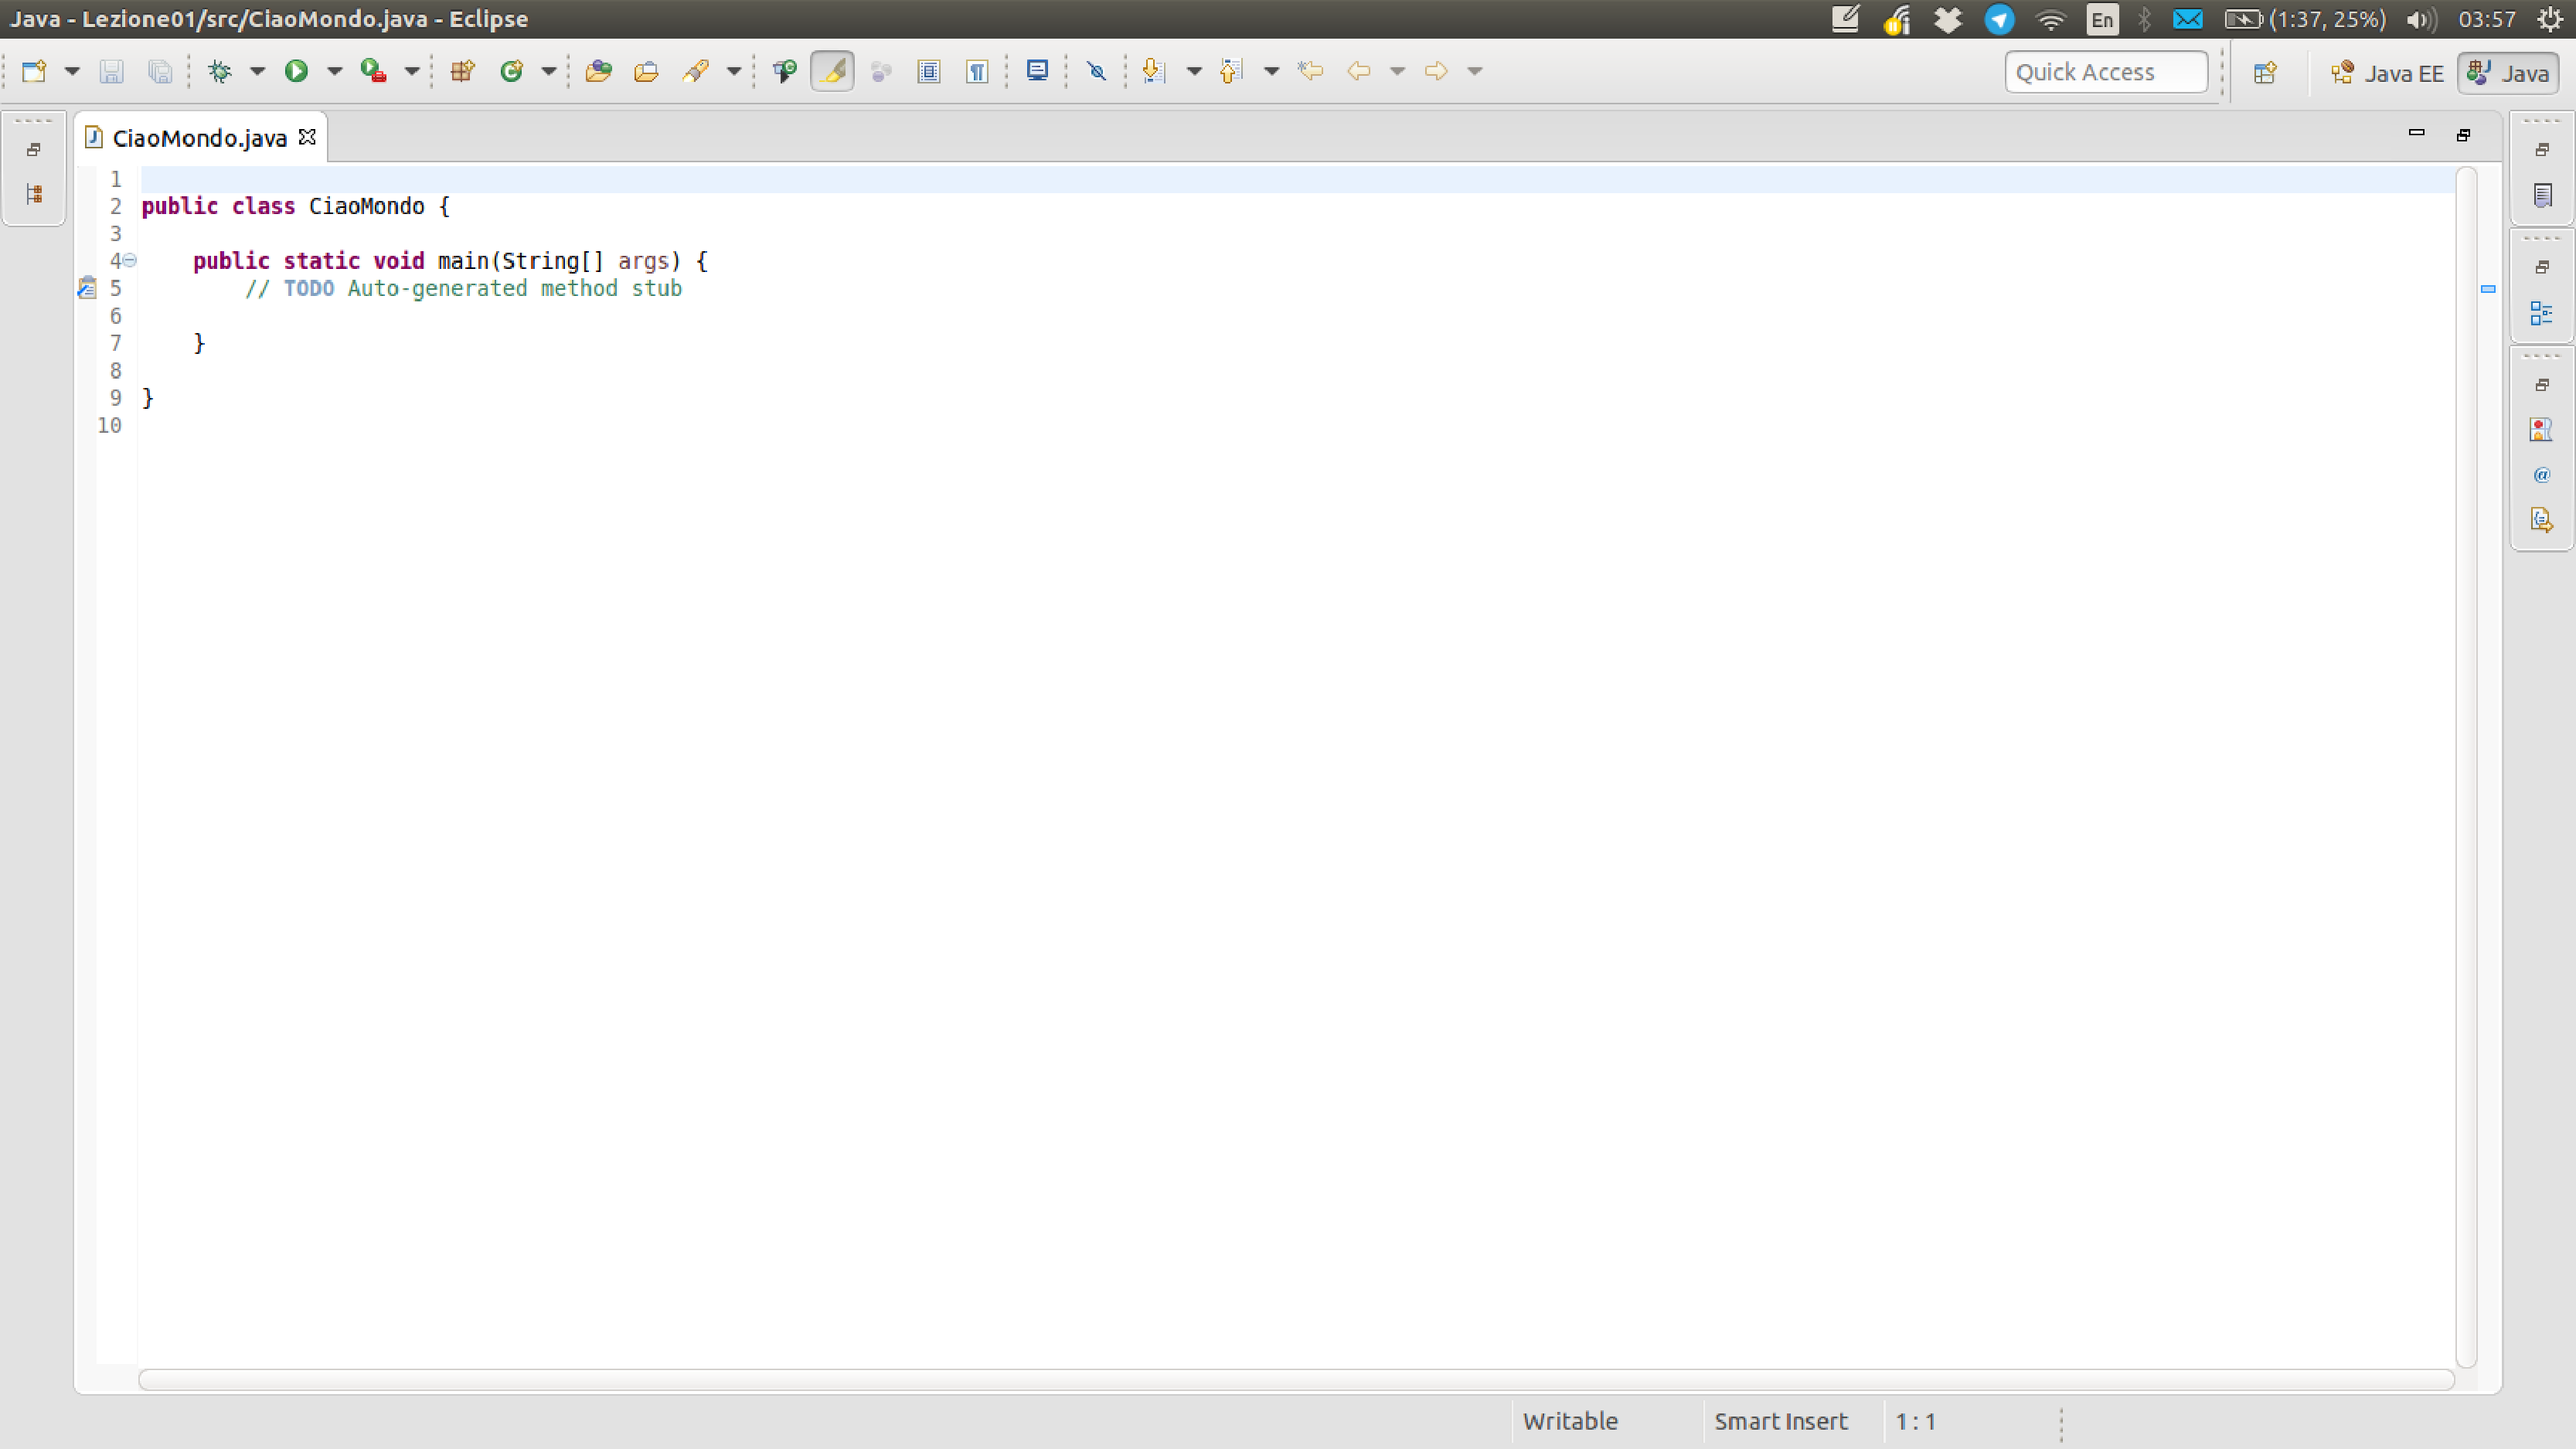
\includepdf[pages={1}]{img/eclipse/code.pdf}
}

% \pgfdeclareimage[height=\paperheight,width=\paperwidth]{suggestion}{img/eclipse/suggestion.png}
% \begin{frame}{Avvio di Eclipse}
%   \begin{center}
%     \pgfuseimage{suggestion}
%   \end{center}
% \end{frame}
{
  \setbeamercolor{background canvas}{bg=}
  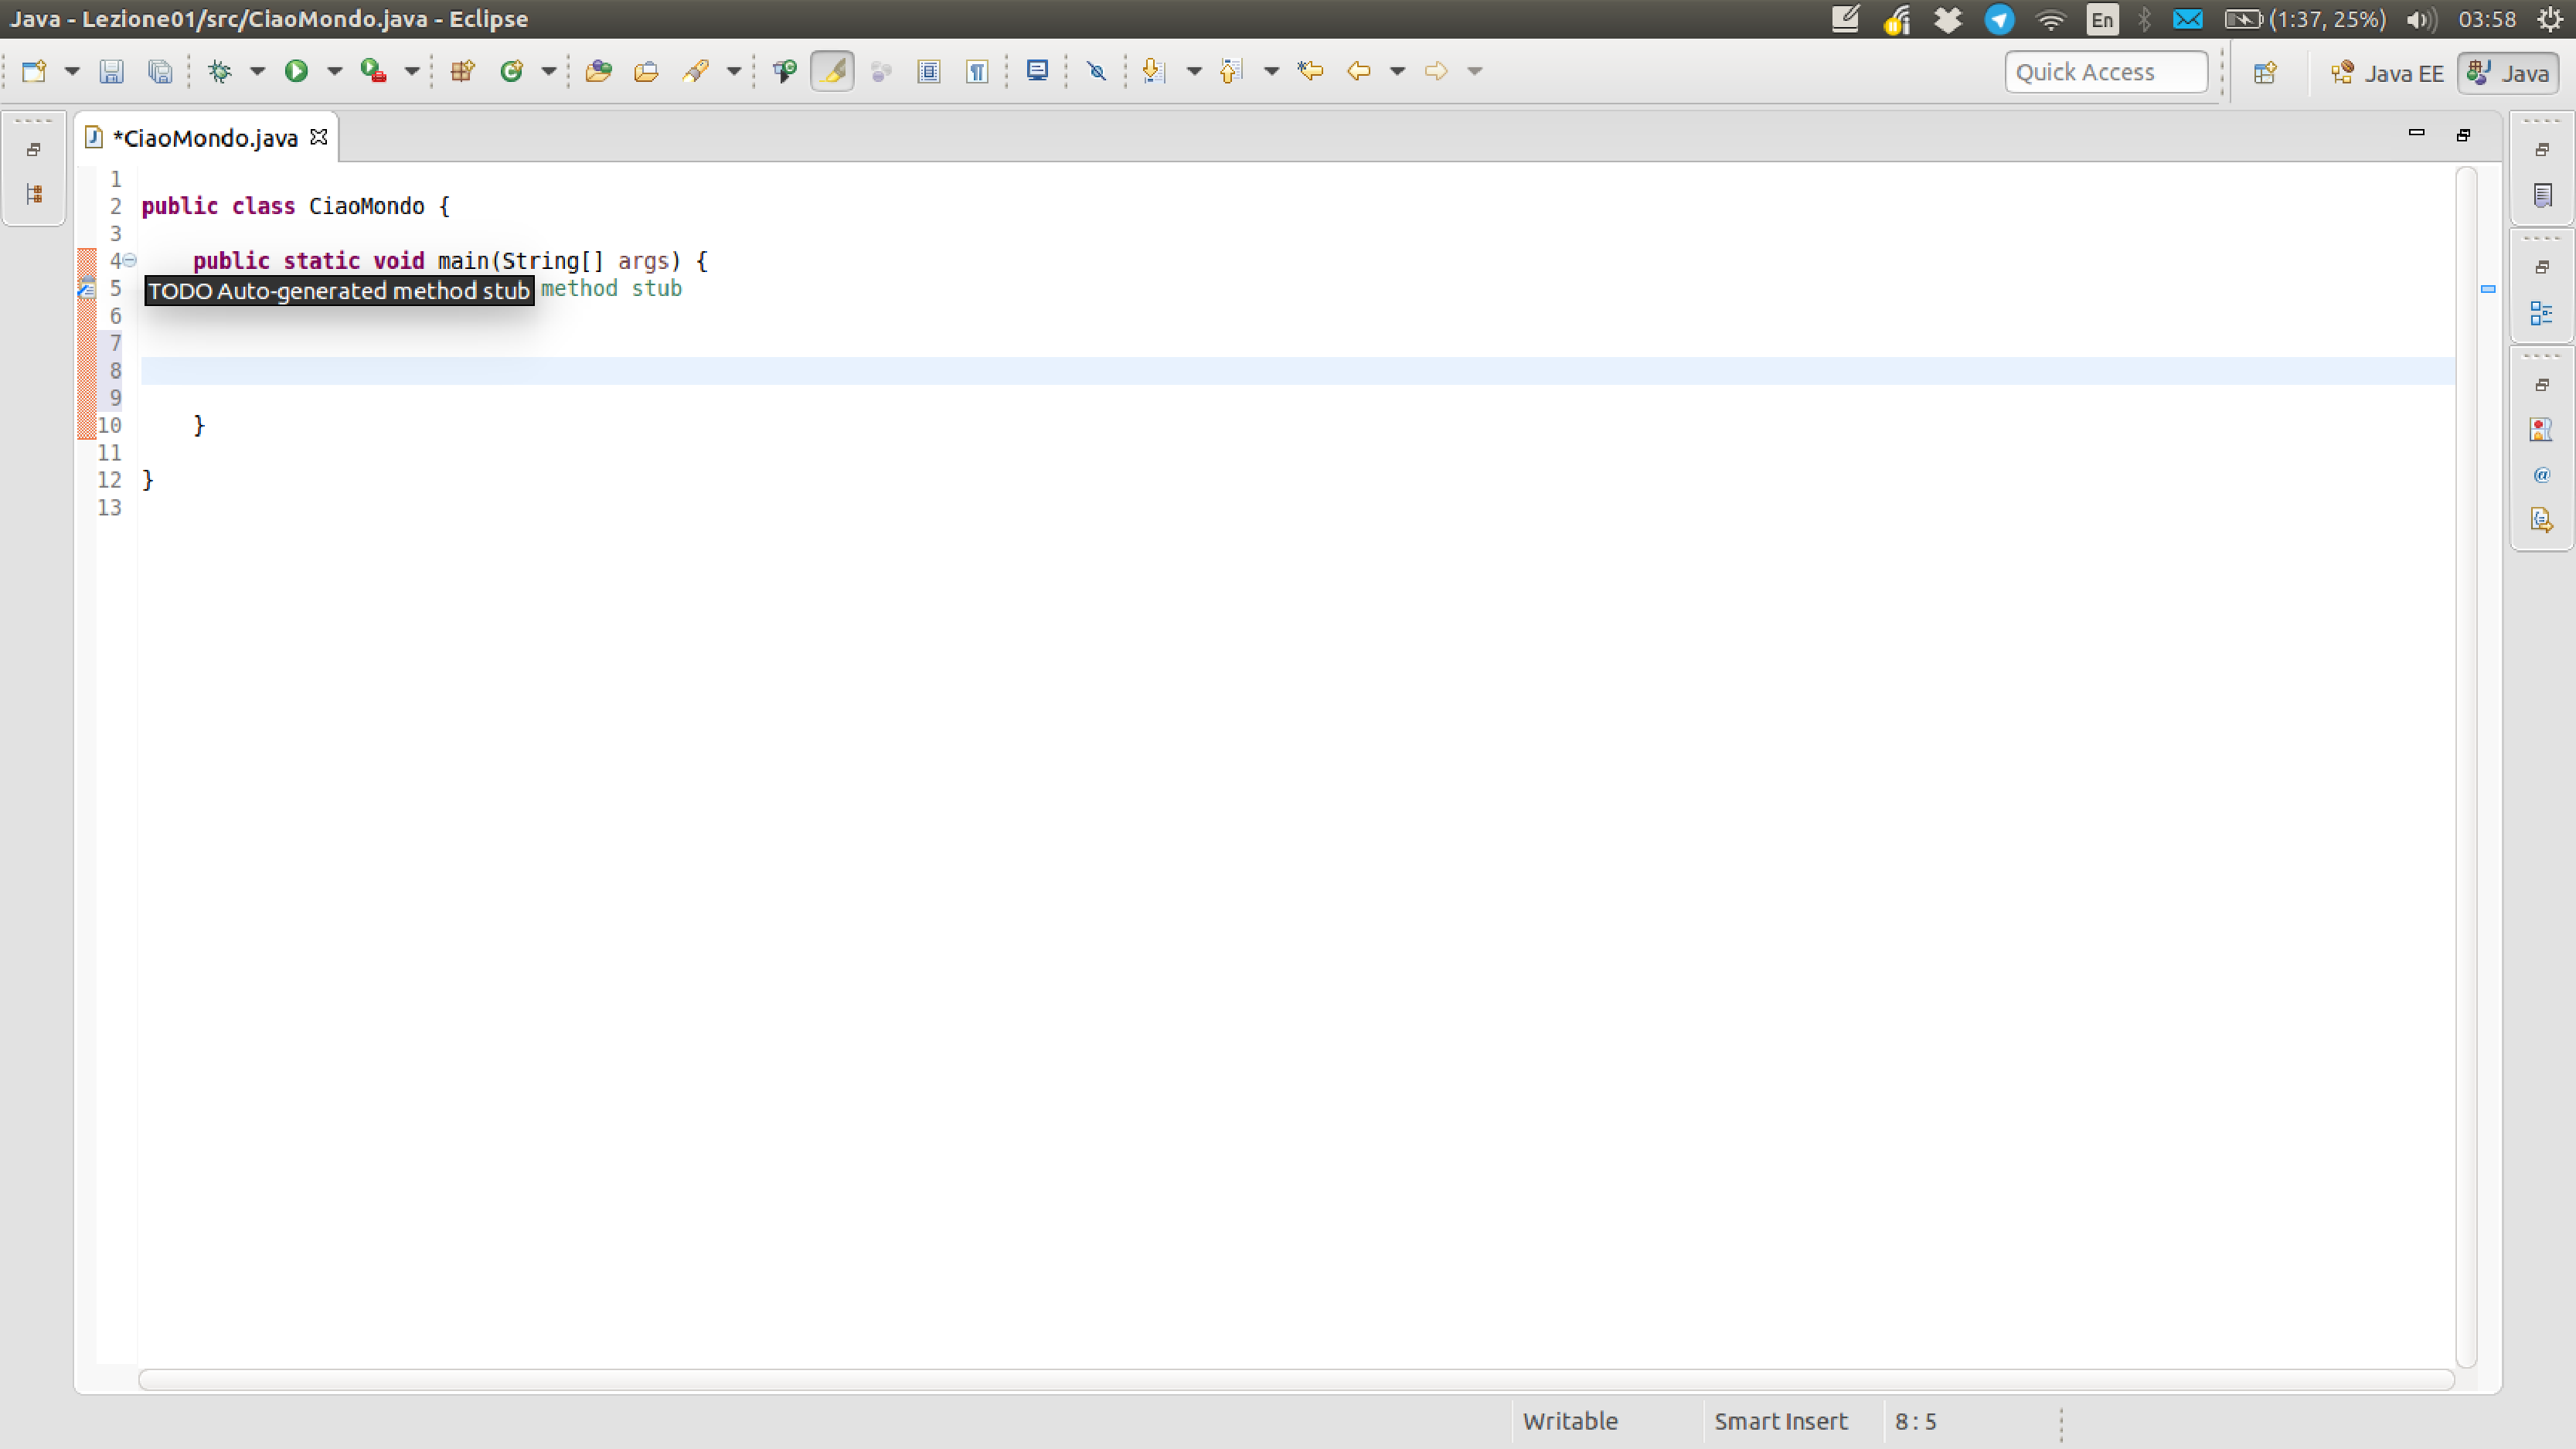
\includepdf[pages={1}]{img/eclipse/suggestion.pdf}
}

\pgfdeclareimage[width=0.5\paperwidth]{big_block}{img/big_block.png}
\begin{frame}{Blocchi (I)}
  \begin{center}
    \pgfuseimage{big_block}
  \end{center}
\end{frame}

\pgfdeclareimage[width=0.5\paperwidth]{big_block_code}{img/big_block_code.png}
\begin{frame}{Blocchi (II)}
  \begin{center}
    \pgfuseimage{big_block_code}
  \end{center}
\end{frame}

\section{Istruzioni Condizionali}
\subsection[Definizione]{Definizione}

\begin{frame}{Istruzione \texttt{if}}
     Le \textbf{istruzioni condizionali} permettono di effettuare operazioni diverse a seconda 
     dei valori delle variabili.
    \begin{algorithmic}[1]
      \If{\alert{condizione}}
	\State istruzione 1
      \Else
	\State istruzione 2
      \EndIf
    \end{algorithmic}
    \alert{condizione} deve essere una \textbf{espressione booleana}.
\end{frame}


\begin{frame}{Istruzione \texttt{if}}
    
    In Java: \\
    \begin{center}
      \texttt{     
	\textbf{if} (\alert{condizione}) \{ \newline
	      comando1 \newline
	    \} \textbf{else} \{ \newline
	      comando2 \newline
	    \} \newline}
    \end{center}

\end{frame}

\section{Esericizi}
\subsection[Esercizi]{Esercizi}

\begin{frame}{Esercizi (I)}
  \begin{itemize}
   \item Scrivete un programma che stampi la canzone popolare inglese ``\emph{99 bottiglie di birra}''
   \item (vedete anche \url{https://esolangs.org/wiki/99_bottles_of_beer})
  \end{itemize}
  \begin{quote}
   «99 bottles of beer on the wall, 99 bottles of beer.\newline
   Take one down, pass it around, 98 bottles of beer on the wall \newline
   99 bottles of beer on the wall, 99 bottles of beer.\newline
   Take one down, pass it around, 98 bottles of beer on the wall  \newline
   ...\newline
   1 bottle of beer on the wall, 1 bottle of beer.\newline
   Take one down, pass it around, no more bottles of beer on the wall\newline
   There no more bottles of beer on the wall, no more bottles of beer.»
  \end{quote}

\end{frame}

\begin{frame}{Esercizi (II)}
  \begin{itemize}
    \item Utilizzando il ciclo \texttt{while} scrivete un programma che dato un 
    intero stampi a schermo la ``tabellina''.
    Ad esempio, se il numero è 7 dovrete stampare a schermo:
    \begin{itemize}
      \item 7*0 = 0
      \item 7*1 = 7
      \item 7*2 = 14
      \item $\dots$
      \item 7*10 = 70
    \end{itemize}
    \item riscrivete il programma precendente usando il ciclo \texttt{for}.
  \end{itemize}
\end{frame}


\begin{frame}{Esercizi (III)}
  \begin{itemize}
   \item Scrivete un programma che calcoli il fattoriale di un numero intero a vostra scelta.
  \end{itemize}

  La definizione del fattoriale è la seguente:
  \begin{equation}
    n! = n \times (n - 1) \times \dots \times 1
  \end{equation}
  quindi il calcolo del fattoriale può essere definito da: 
  \begin{center}
    \begin{minipage}{8cm}
      \begin{algorithmic}[1]
	\State $fatt \gets ?$ \Comment Quale valore va messo qui?
	\For{$i \gets 1$ to $N$}
	  \State $fatt \gets fatt \times i$ 
	\EndFor
      \end{algorithmic}
   \end{minipage}
  \end{center}

\end{frame}

\begin{frame}{Esercizi (IV)}
  \begin{itemize}
    \item Scrivere un programma che stampi i valori della serie di Fibonacci minori di 10000.
    La serie di Fibonacci \`e definita da:
    \begin{equation*}
      \left\{\begin{aligned}
	  & x_0 = 1\\
	  & x_1 = 1\\
	  & x_{n+1} = x_{n} + x_{n-1}
      \end{aligned}\right.
    \end{equation*}
  \end{itemize}

\end{frame}


\begin{frame}{Esercizi (V)}
  \begin{itemize}
    \item Scrivere un programma che usi il metodo per il calcolo della radice quadrata di Newton.
    
    \begin{equation*}
      \left\{\begin{aligned}
	  & x_0 = 0.5\\
	  & x_{n +1} = 0.5 \cdot {x_n} (3  - zx^2_n)
      \end{aligned}\right.
    \end{equation*}
    \begin{equation*}
     \lim_{n \to \infty} x_{n} = \sqrt{z}
    \end{equation*}
  \end{itemize}
  
  Il programma deve calcolare la serie definita sopra fino a che l'errore $\varepsilon_{n} = |x^{2}_{n} - z|$,
  non è più piccolo di $10^{-3}$. Per il valore assoluto utilizzate la funzione \texttt{Math.\Blue{abs()}}.

\end{frame}

\begin{frame}{Esercizi (VI)}
  \begin{itemize}
    \item Metodo della bisezione
  \end{itemize}
  \begin{tiny}
    \url{https://ece.uwaterloo.ca/~dwharder/NumericalAnalysis/10RootFinding/bisection/bisection.gif}
  \end{tiny}

  \begin{scriptsize}
    \begin{center}
      \begin{minipage}{8cm}
	\begin{algorithmic}[1]
	  \Require Function $f$, endpoint values $a, b$, tolerance $\varepsilon$, maximum iterations $N_{MAX}$
		   $a < b$, either $f(a) < 0$ and $f(b) > 0$ or $f(a) > 0$ and $f(b) < 0$
	  \Ensure value which differs from $a$ root of $f(x)=0$ by less than $\varepsilon$
    
	  \State $N \gets 1$
	  \While{$N \leq N_{MAX}$}
	    \State $c \gets (a + b)/2$
	    \If{$f(c) = 0 \lor (b – a)/2 < \varepsilon$}
	      \State \texttt{\textbf{print}}(c)
	      \State \Return;
	    \EndIf
	    \State $N \gets N + 1$
	    \If{$sign(f(c)) = sign(f(a))$}
	      \State $a \gets c$
	    \Else 
	      \State $b \gets c$
	    \EndIf
	  \EndWhile
	  \State \texttt{\textbf{print}}(Non ho trovato risultati)
	\end{algorithmic}
      \end{minipage}
    \end{center}
  \end{scriptsize}

\end{frame}

\begin{frame}{Esercizi (VII)}
  Test di primalità
  \begin{itemize}
    \item Scrivere un programma che, dato un intero positivo, verifichi se quel numero è primo oppure no.
  \end{itemize}

   Un numero $n \in \mathbb{N}, n > 1$ \`e \textbf{primo} se e solo se \`e divisibile solo per $1$ e per
   se stesso.
\end{frame}

% \appendix
% \section*{Backup}
% \begin{frame}
\begin{Huge}
Backup 
\end{Huge}
\end{frame}


\end{document}
